\sloppy
\chapter{FUNKCIONALNI ZAHTJEVI}

\sloppy
\section*{Kontrola verzija}

U par rečenica opisati koji članovi tima su učestvovali u kreiranju ovog poglavlja.

\noindent Emir Duvnjak - FZ1

\noindent Tarik Hastor - FZ2

\noindent Zakir Šehić - FZ3 i FZ4


\sloppy  
\section{FZ1: Pregled i uređivanje predstava}  

\sloppy  
\subsection{Opis funkcionalnog zahtjeva}  
\begin{itemize}  
    \item \textbf{Poslovni proces}: Pregled i filtriranje trenutnih predstava  
    \item \textbf{Vrste korisnika}: Administrator, Registrovani korisnik.  
    \item \textbf{Scenariji korištenja}:  
        \begin{enumerate}  
            \item \textbf{Promijenjen termin predstave-korisnik potvrđuje rezervaciju:} \\
            Nakon pregleda detalja predstave (datum, vrijeme, glumci) administrator mijenja termin predstave i šalje obavještenje korisniku koji prihvata izmjenu odabranog termina i potvrđuje rezervaciju  
            
            \item \textbf{Promijenjen termin predstave-korisnik odustaje od rezervacije:} \\
            Nakon pregleda detalja predstave administrator mijenja termin predstave i šalje obavještenje korisniku koji ne prihvata izmjenu odabranog termina i odustaje od rezervacije
  
            \item \textbf{Administrator odustaje od promjene termina:} \\
            Nakon detaljnog pregleda detalja predstave administrator odustaje od promjene termina  
        \end{enumerate}
    \item \textbf{UML dijagram aktivnosti}: Prikazan na slici \ref{fig:fz1} 
\end{itemize}   
\begin{figure}[H]
    \centering
    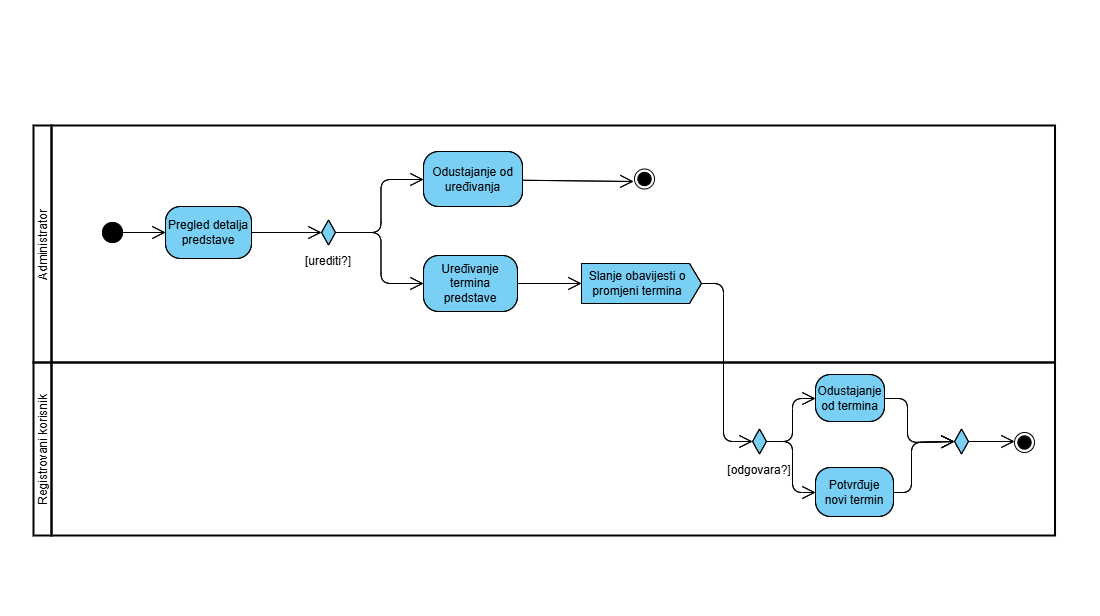
\includegraphics[width=1\textwidth]{Slike/Fz1.png}
    \caption{UML dijagram aktivnosti "Pregled i uređivanje predstava"}
    \label{fig:fz1}
\end{figure}

\sloppy  
\subsection{Dizajn korisničkih interfejsa}  
\begin{itemize}  
    \item \textbf{Prototip interfejsa}: Prikaz aktivnih predstava s opcijom uređivanja termina za administratore kao i pregleda izmijenjenih termina i aktivnih predstava za korisnike. Slike: \ref{fig:adminView} i \ref{fig:userView}
    \item \textbf{Opis scenarija}:  
        \begin{itemize}  
            \item Administrator pomiče predstavu u kalendaru i šalje obavijest korisnicima.  
            \item Korisnik pregleda ažurirani raspored i potvrđuje novi termin.  
        \end{itemize}  
\end{itemize}   

\begin{figure}[H]
    \centering
    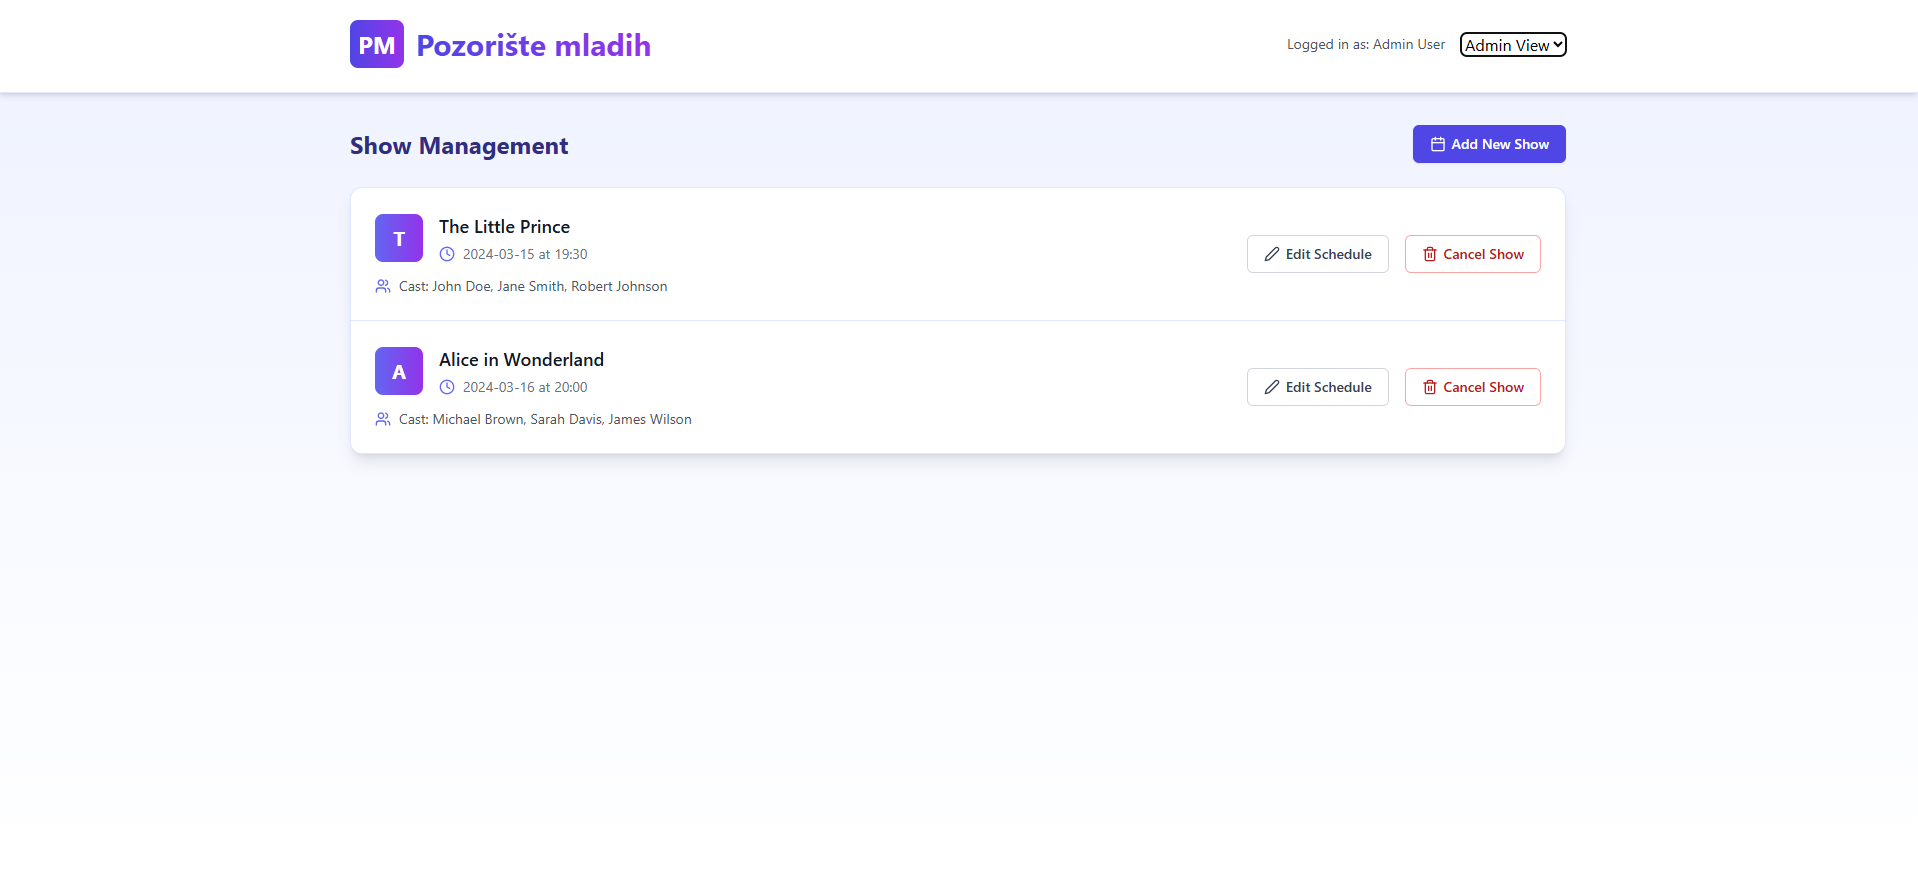
\includegraphics[width=1\textwidth]{Slike/adminView.PNG}
    \caption{Prototip interfejsa administratora za "Pregled i uređivanje predstava"}
    \label{fig:adminView}
\end{figure} 

\begin{figure}[H]
    \centering
    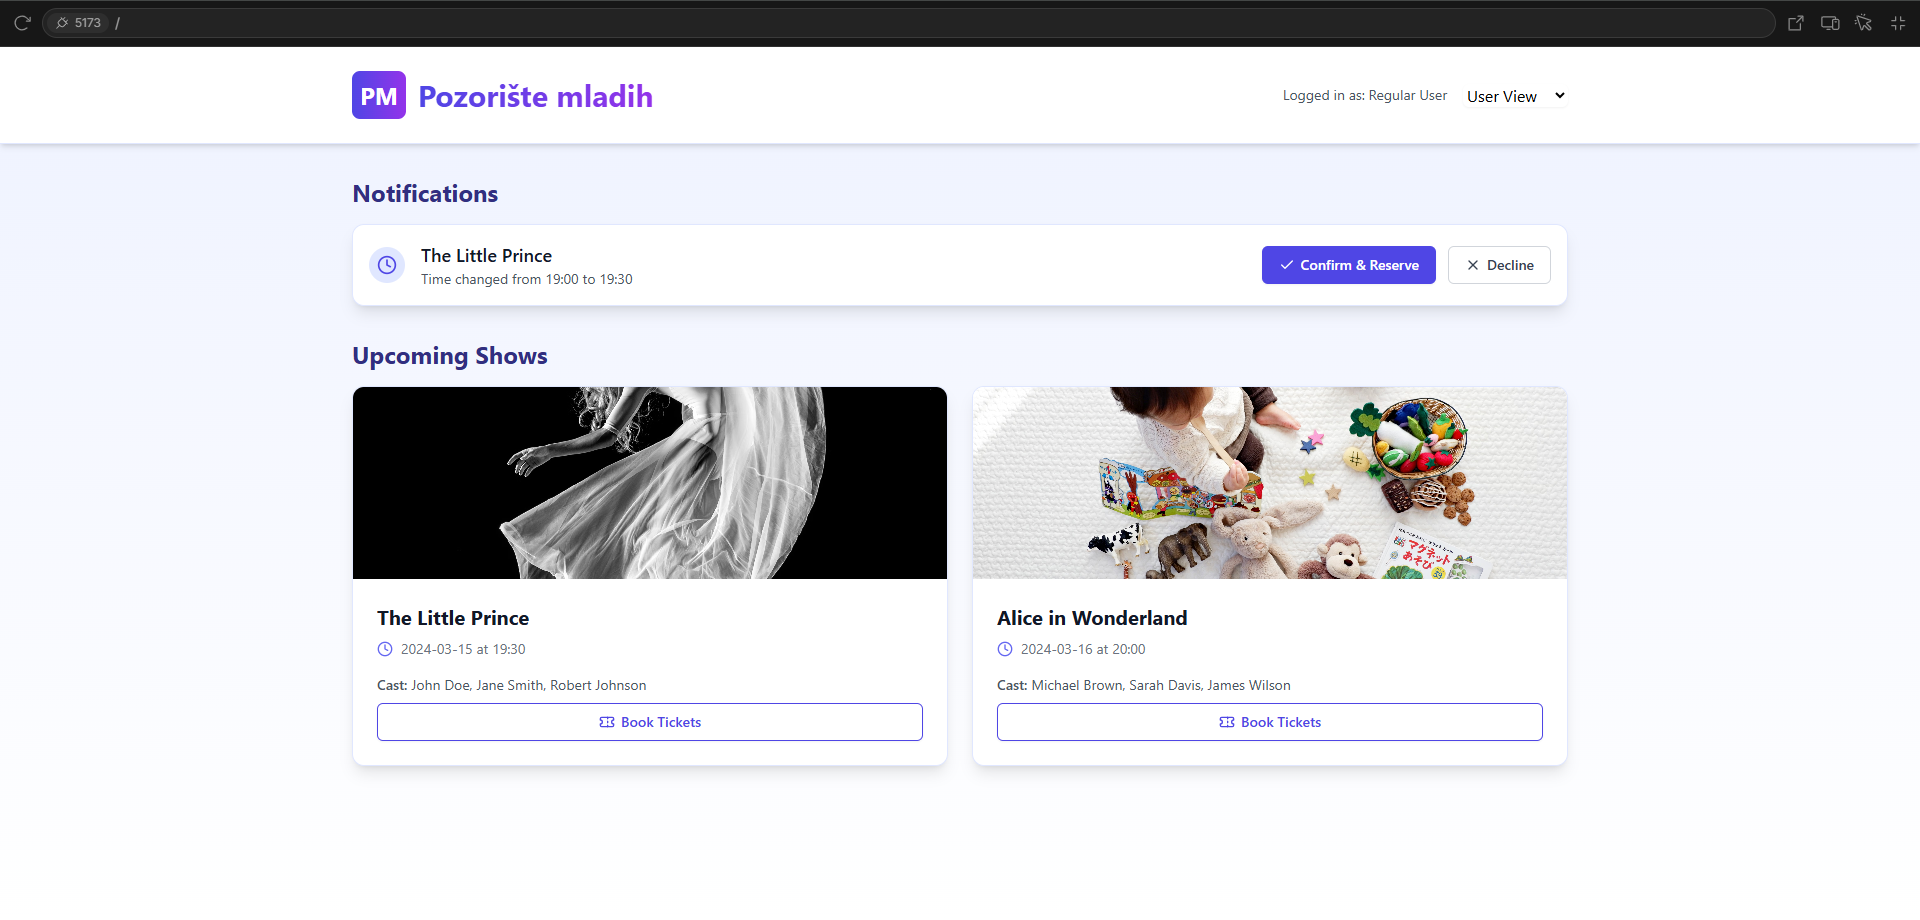
\includegraphics[width=1\textwidth]{Slike/userView.PNG}
    \caption{Prototip interfejsa korisnika za pregled izmijenjenih termina i aktivnih predstava}
    \label{fig:userView}
\end{figure}
\subsection{Bolt \textit{promptovi}}
\begin{enumerate}  
            \item \textbf{Prvi \textit{prompt}:}
            
            \textit{"Design a modern and user-friendly webpage for managing show schedules. The design should include distinct sections or interfaces for administrators and registered users, reflecting the following functionalities:}
        
            \textit{Administrator Interface:}
            
            \textit{Show Details View: A section where administrators can view a list of shows with their details, including date, time, and actors.
            Edit Functionality: An option (like an 'Edit' button) for each show that allows administrators to modify its schedule (specifically the time).
            Notification System: After editing a show's time, the system should prompt the administrator to send a notification about this change to all registered users.
            Cancel Edit Option: During the editing process, administrators should have an option to cancel their changes.}
            \textit{Registered User Interface:
            Notification Display: A section where registered users can view notifications about changes to show times.
            Updated Schedule View: Users should be able to see the updated schedule of shows.
            Confirmation/Rejection: For each notification about a time change, users should have clear options to either 'Confirm' the new time or 'Decline' it.
            The overall design should be clean, modern, and easy to navigate for both administrators and registered users. Consider using a visually appealing layout and intuitive controls for each action."}


            
            \item \textbf{Drugi \textit{prompt}:}
            
            \textit{"Building upon the previous request for a webpage design to manage show schedules, please make the following enhancements:}

            \textit{Modern Design  Youth Theater Theme: Update the overall design to be more modern and visually appealing, with a style that is suitable for a youth theater. Consider using a vibrant color palette and playful design elements to create an energetic and engaging user experience.}
            
            \textit{Notification Specificity: When displaying notifications to registered users about show time changes, ensure that each notification clearly states which show the time change is for.
            Reservation Integration: For registered users, when they click the 'Confirm' button on a notification regarding a show time change, instead of just confirming, the action should redirect them to a reservation or booking screen specifically for that show and the new time. This will allow them to immediately proceed with booking tickets for the updated schedule."}


  
            \item \textbf{Treći \textit{prompt}:}
            
            \textit{Please fix the image on the Alice in Wonderland page. Additionally, in the admin section, add functionality to modify the date as well as the time of an event. There should also be an option to cancel the entire show. Ensure all these changes are reflected for the user. Furthermore, when viewing as a regular user, the display should say 'Logged in as User' instead of 'admin'.}
        \end{enumerate}

\sloppy  
\section{FZ2: \textit{Online} prodaja i rezervacija karata s višestrukim načinima plaćanja}  



\sloppy  
\subsection{Opis funkcionalnog zahtjeva}  
\begin{itemize}  
    \item \textbf{Poslovni proces}: Online prodaja i rezervacija karata s višestrukim načinima plaćanja. 
    \item \textbf{Vrste korisnika}: Gost, Registrovani korisnik, sistem  
    \item \textbf{Scenariji korištenja}:  
        \begin{enumerate}  
            \item Neregistrovani korisnik pregleda predstave, dodaje željenu u korpu i rezerviše unosom podataka za rezervaciju. Sistem obavještava o uspješnosti rezervacije.  
            \item Registrovani korisnik pregleda dostupne predstave, dodaje željenu u korpu i odabira rezervaciju sa plaćanjem te bira načina plaćanja (kreditna kartica, \textit{Google Pay, PayPal}). Sistem obavještava o uspješnosti rezervacije.  
            \item Registrovani korisnik pregleda dostupne predstave, dodaje željenu u korpu i odabira rezervaciju bez plaćanja gdje se njegovi podaci automatski unose. Sistem obavještava o uspješnosti rezervacije.  
        \end{enumerate}  
    \item \textbf{UML dijagram aktivnosti}: Prikazan na slici \ref{fig:fz2}.  
\end{itemize}  
\begin{figure}[H]
    \centering
    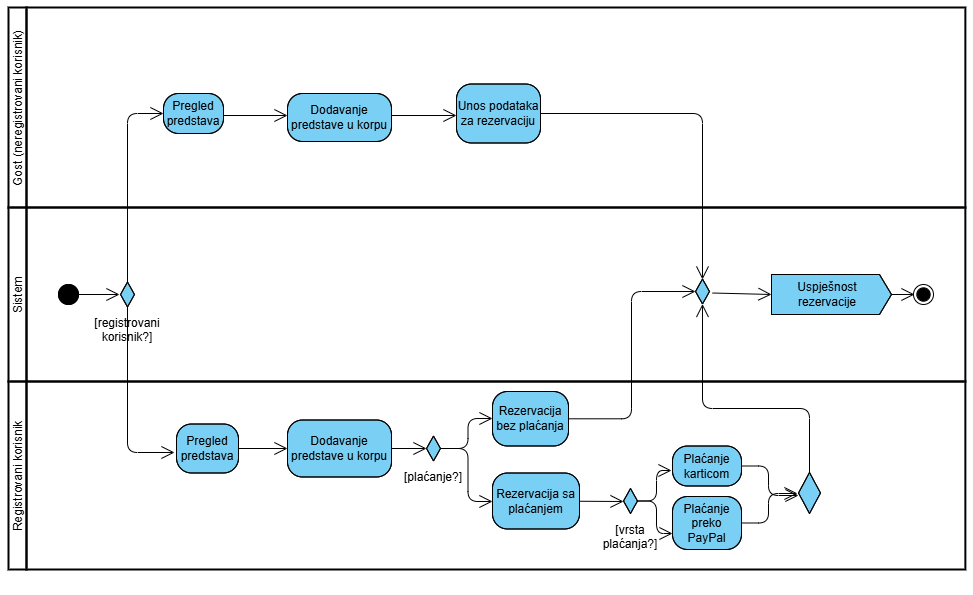
\includegraphics[width=0.8\textwidth]{Slike/Fz2.png}
    \caption{UML dijagram aktivnosti "\textit{Online} prodaja i rezervacija karata"}
    \label{fig:fz2}
\end{figure}
\sloppy  
    \textbf{Opis scenarija}:  
        \begin{itemize}  
            \item Korisnik bira predstavu, odabire sjedište klikom na mapu, te odabire način plaćanja.  
            \item Gost mora unijeti osnovne podatke (ime, e-mail) za rezervaciju.  
        \end{itemize}  
\subsection{Dizajn korisničkih interfejsa}  
\begin{itemize}  
    \item \textbf{Prototip interfejsa}: Interfejsi koji odgovara prethodno navedenim zahtjevima prikazani su na slikama \ref{fig:userfront}, \ref{fig:userselect}, \ref{fig:userview}, \ref{fig:usercheckout}, \ref{fig:userfrontlist},  \ref{fig:guesthome}, \ref{fig:questcheck}
\begin{figure}[H]
    \centering
    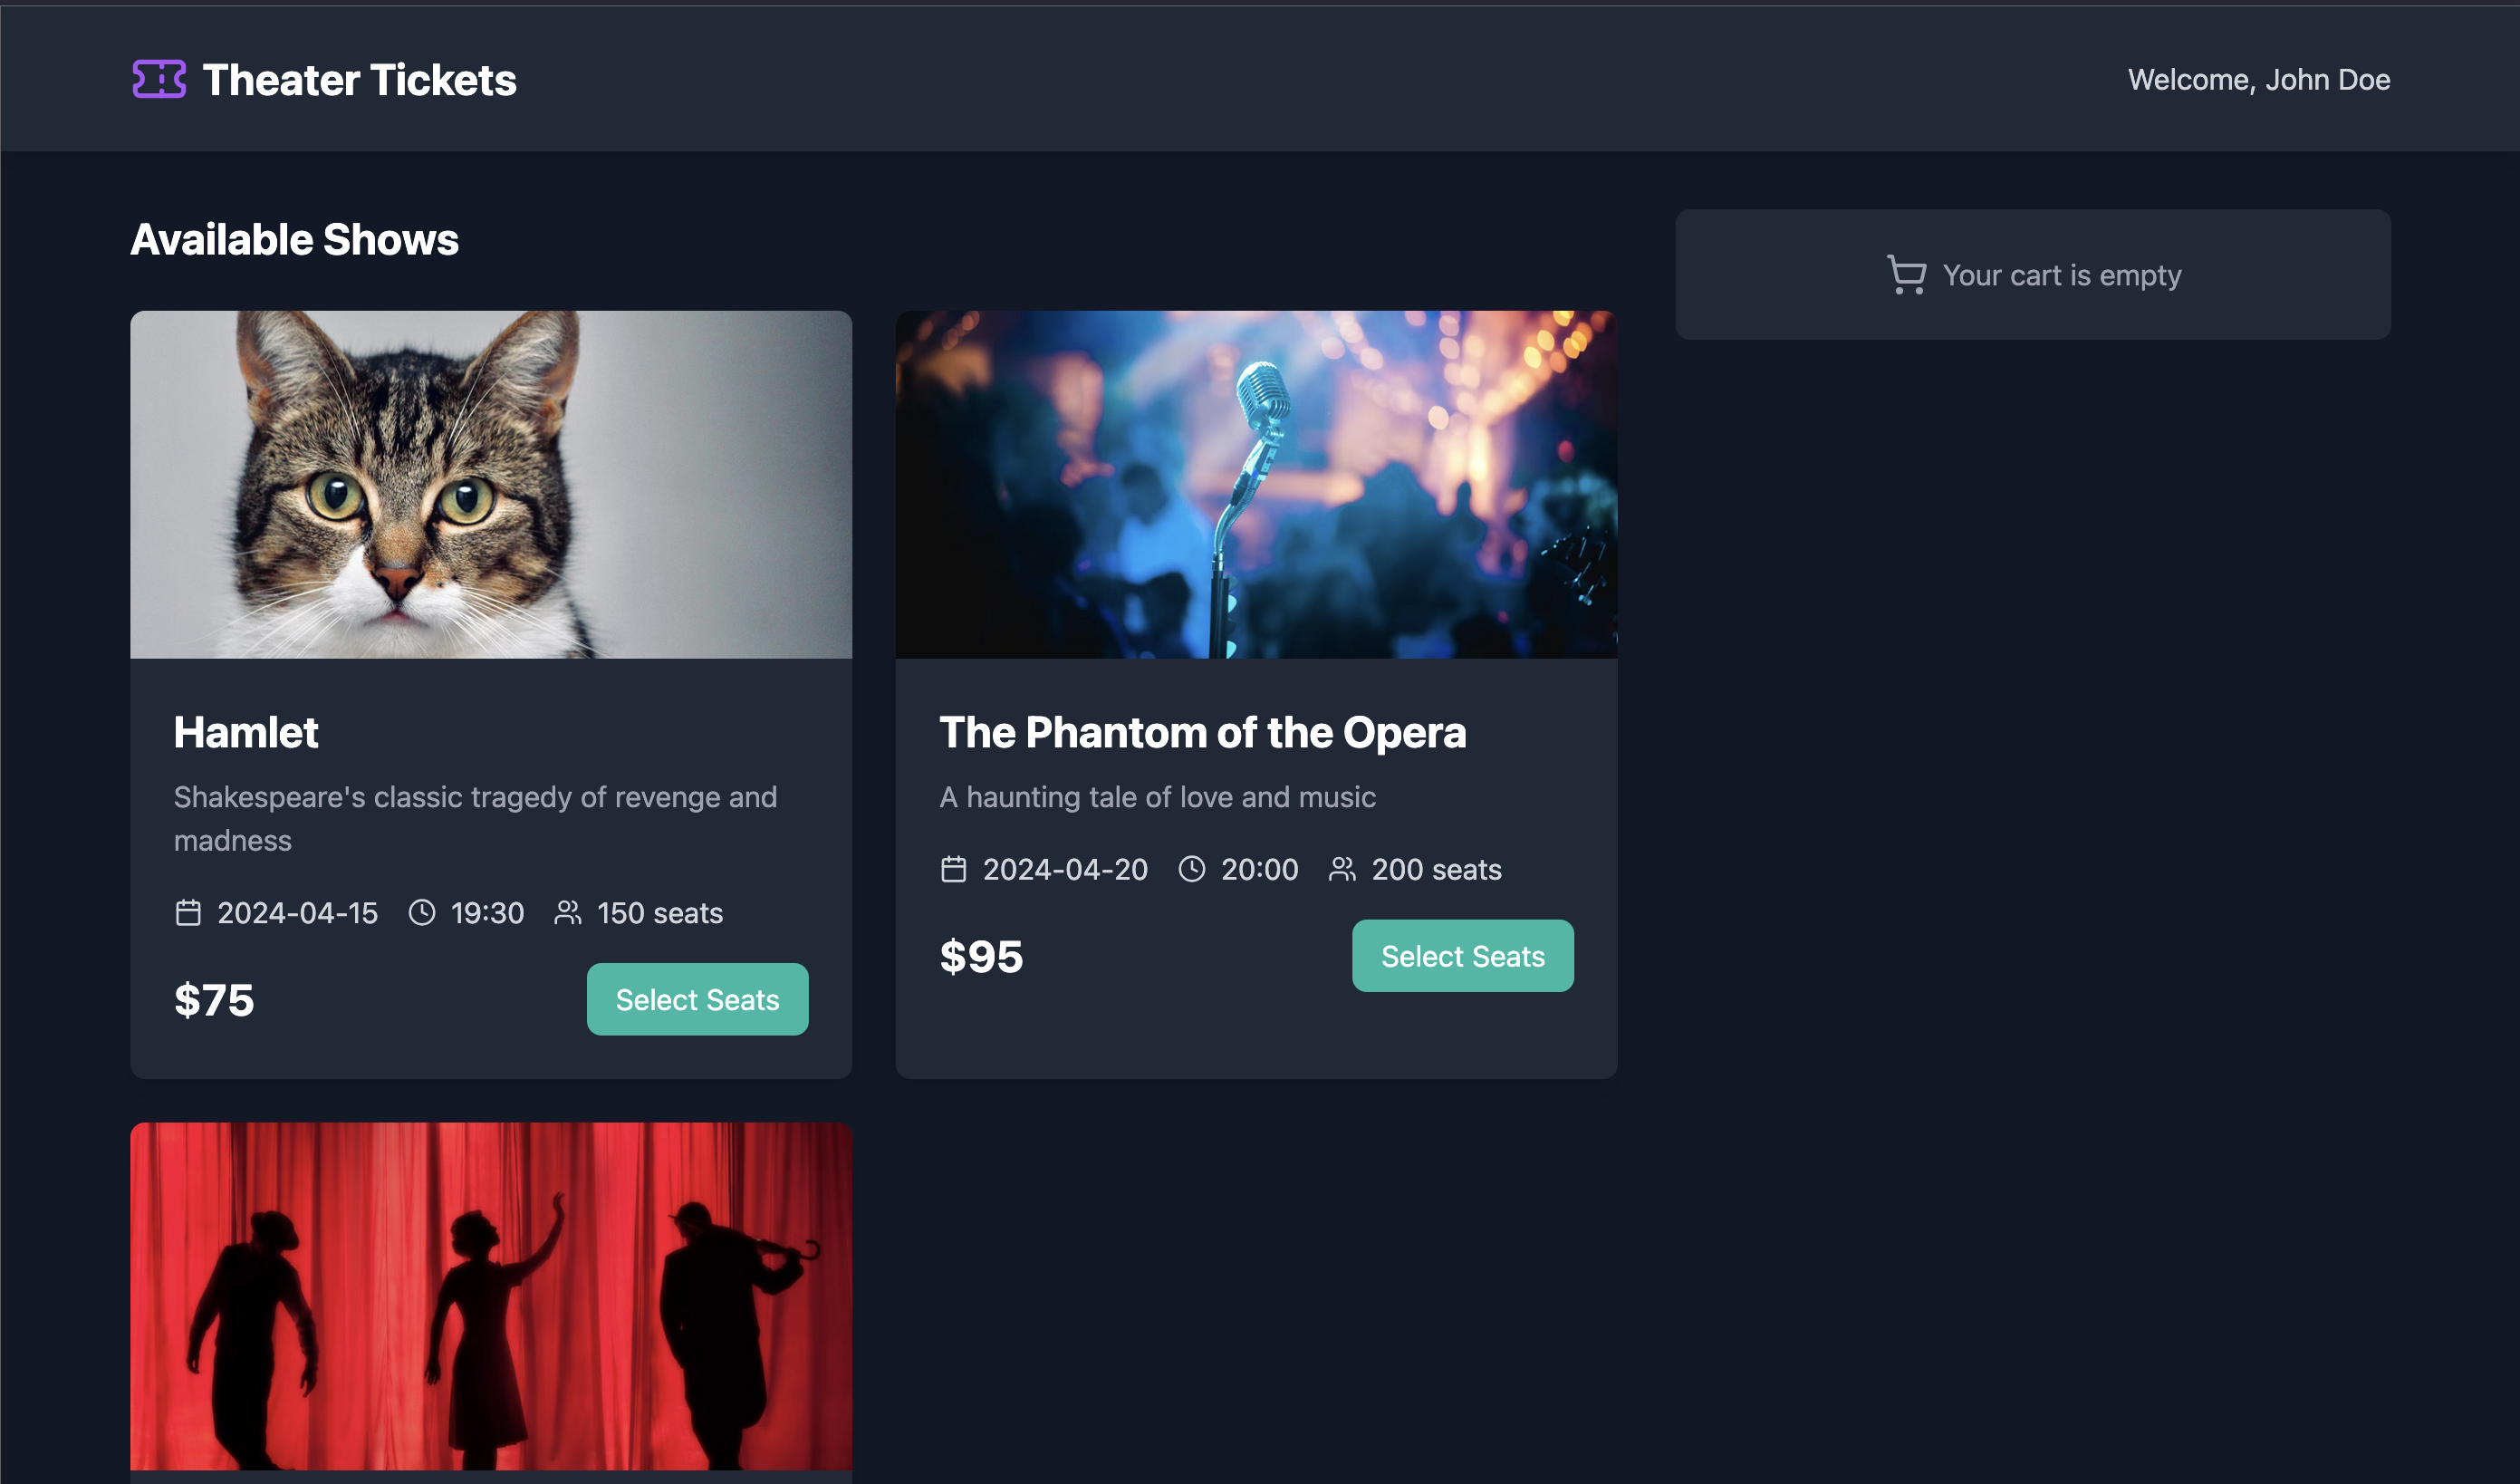
\includegraphics[width=0.9\textwidth]{Slike/FZ2ui/userfront.png}
    \caption{Prototip interfejsa korisnika za pregled predstava}
    \label{fig:userfront}
\end{figure} 
\begin{figure}[H]
    \centering
    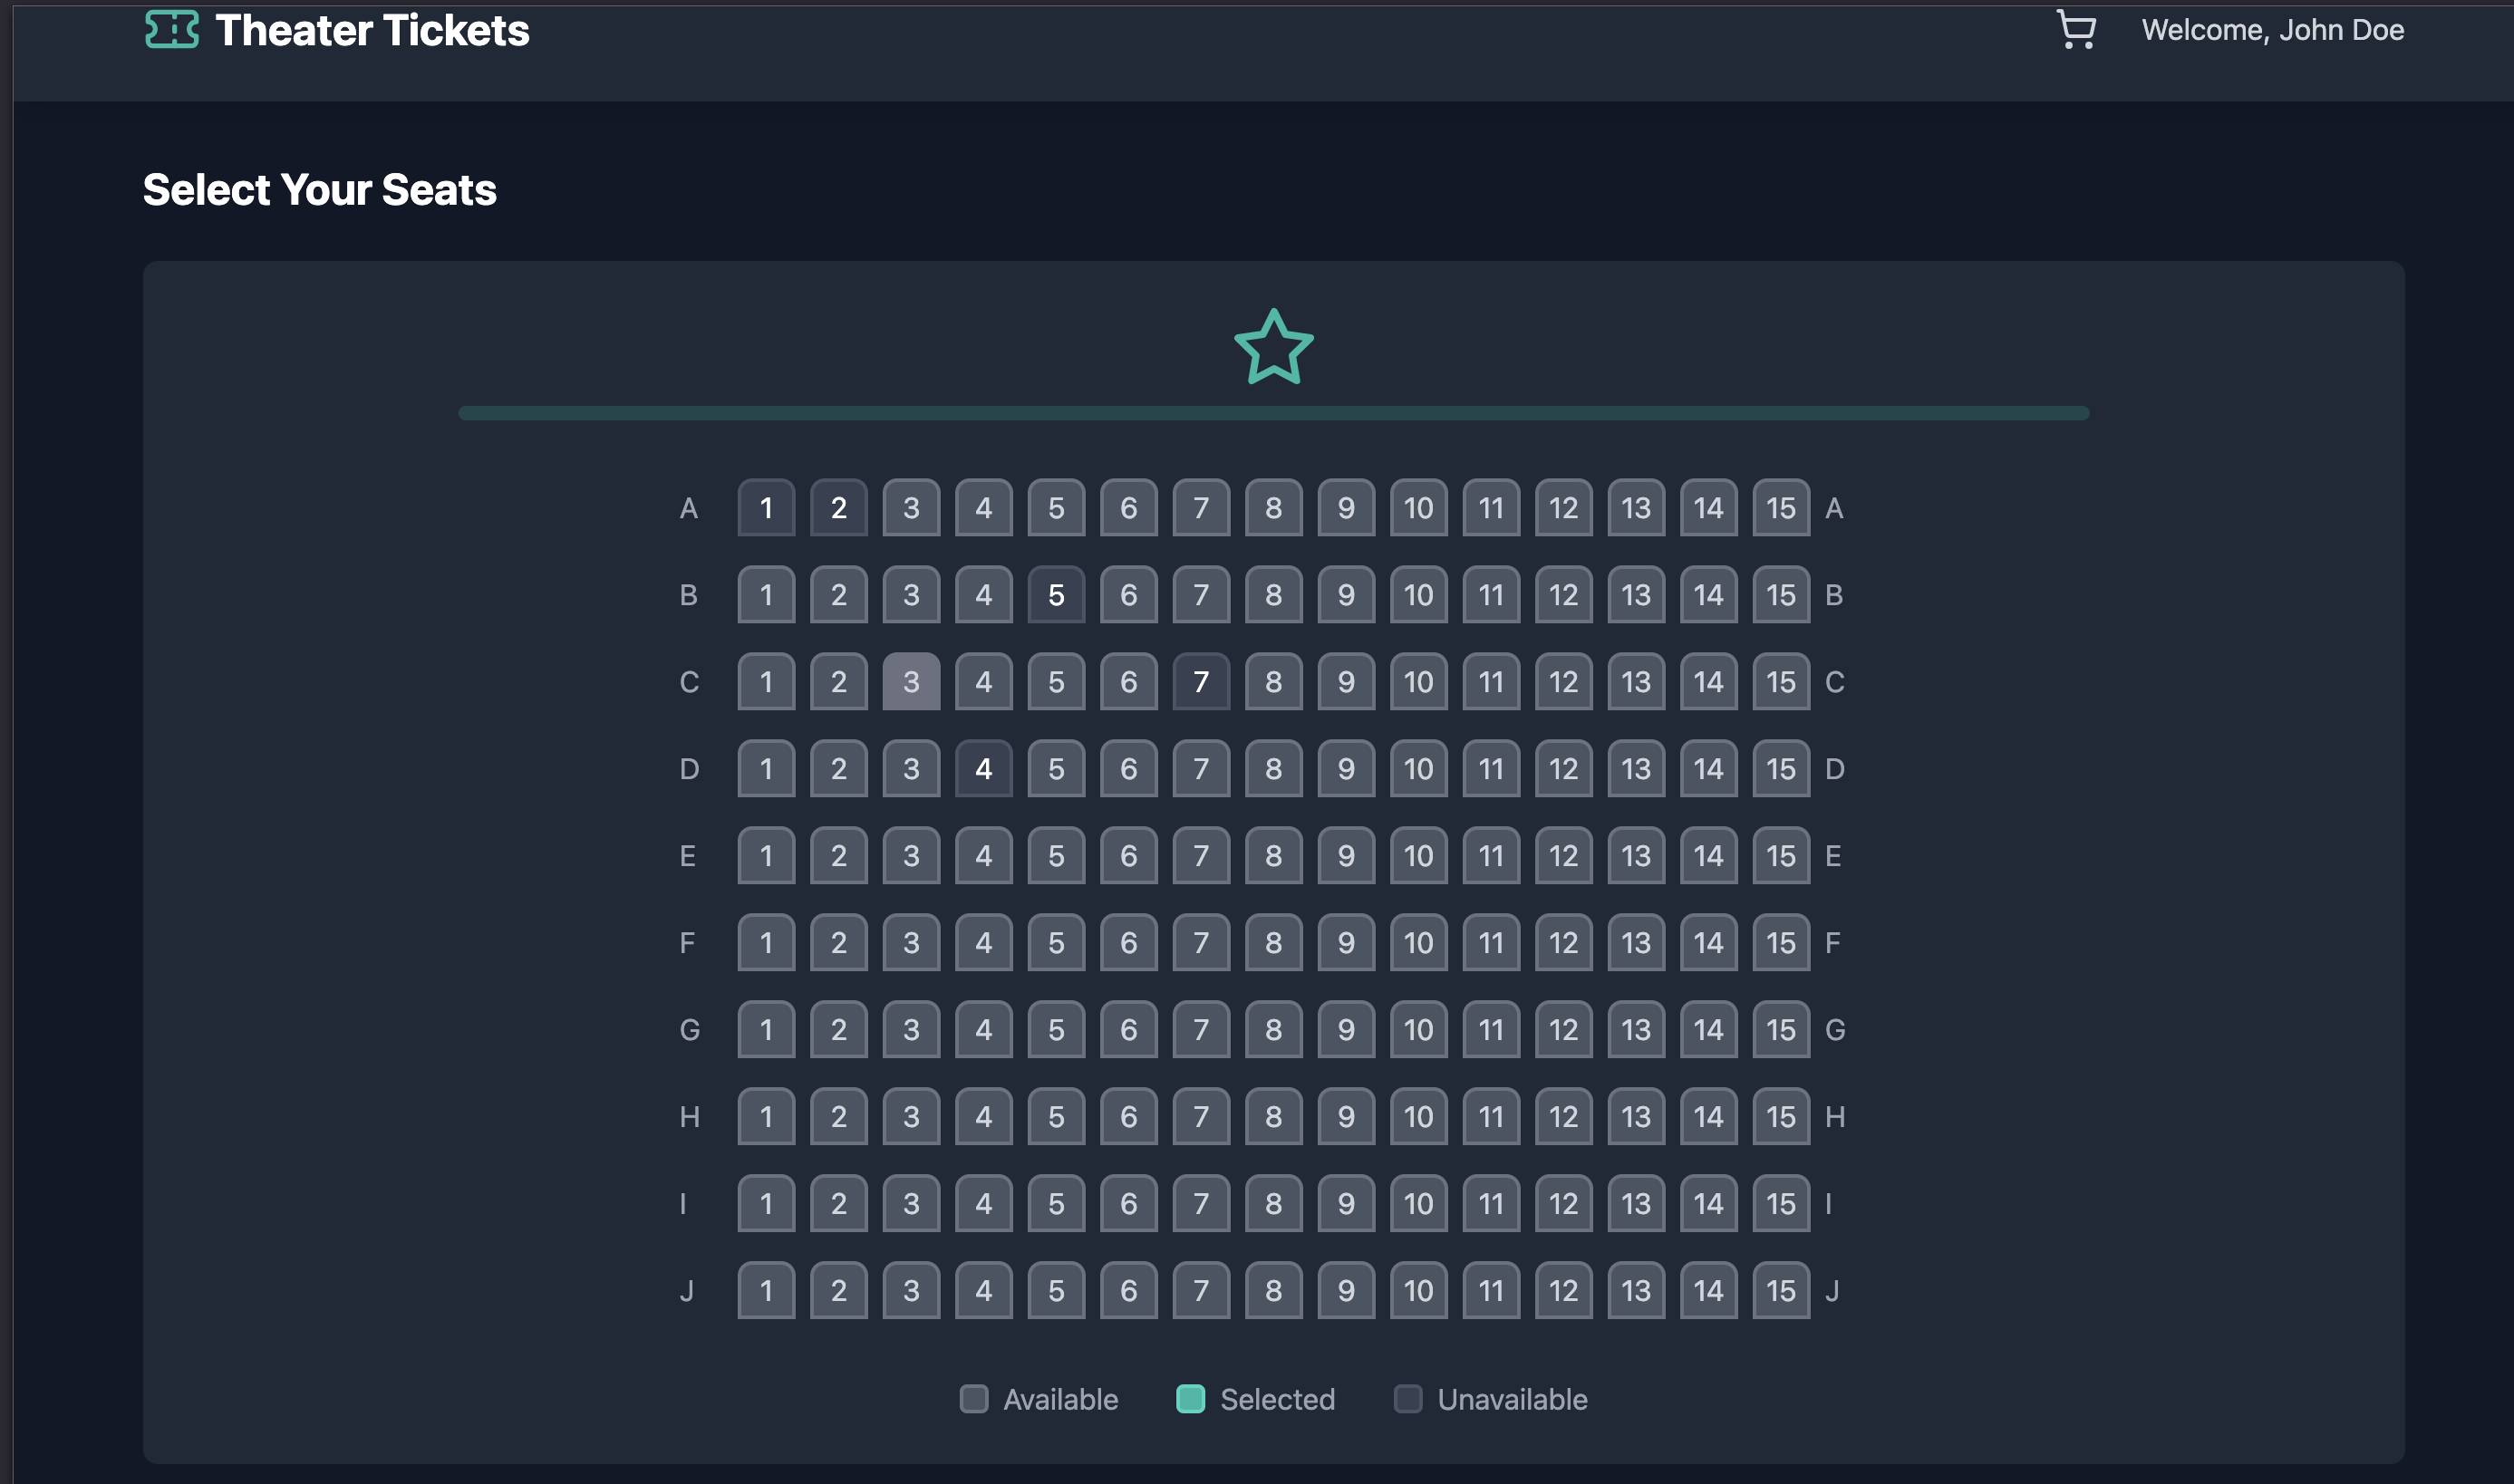
\includegraphics[width=0.9\textwidth]{Slike/FZ2ui/userselect.png}
    \caption{Prototip interfejsa korisnika za pregled i odabir slobodnih mjesta}
    \label{fig:userselect}
\end{figure}
\begin{figure}[H]
    \centering
    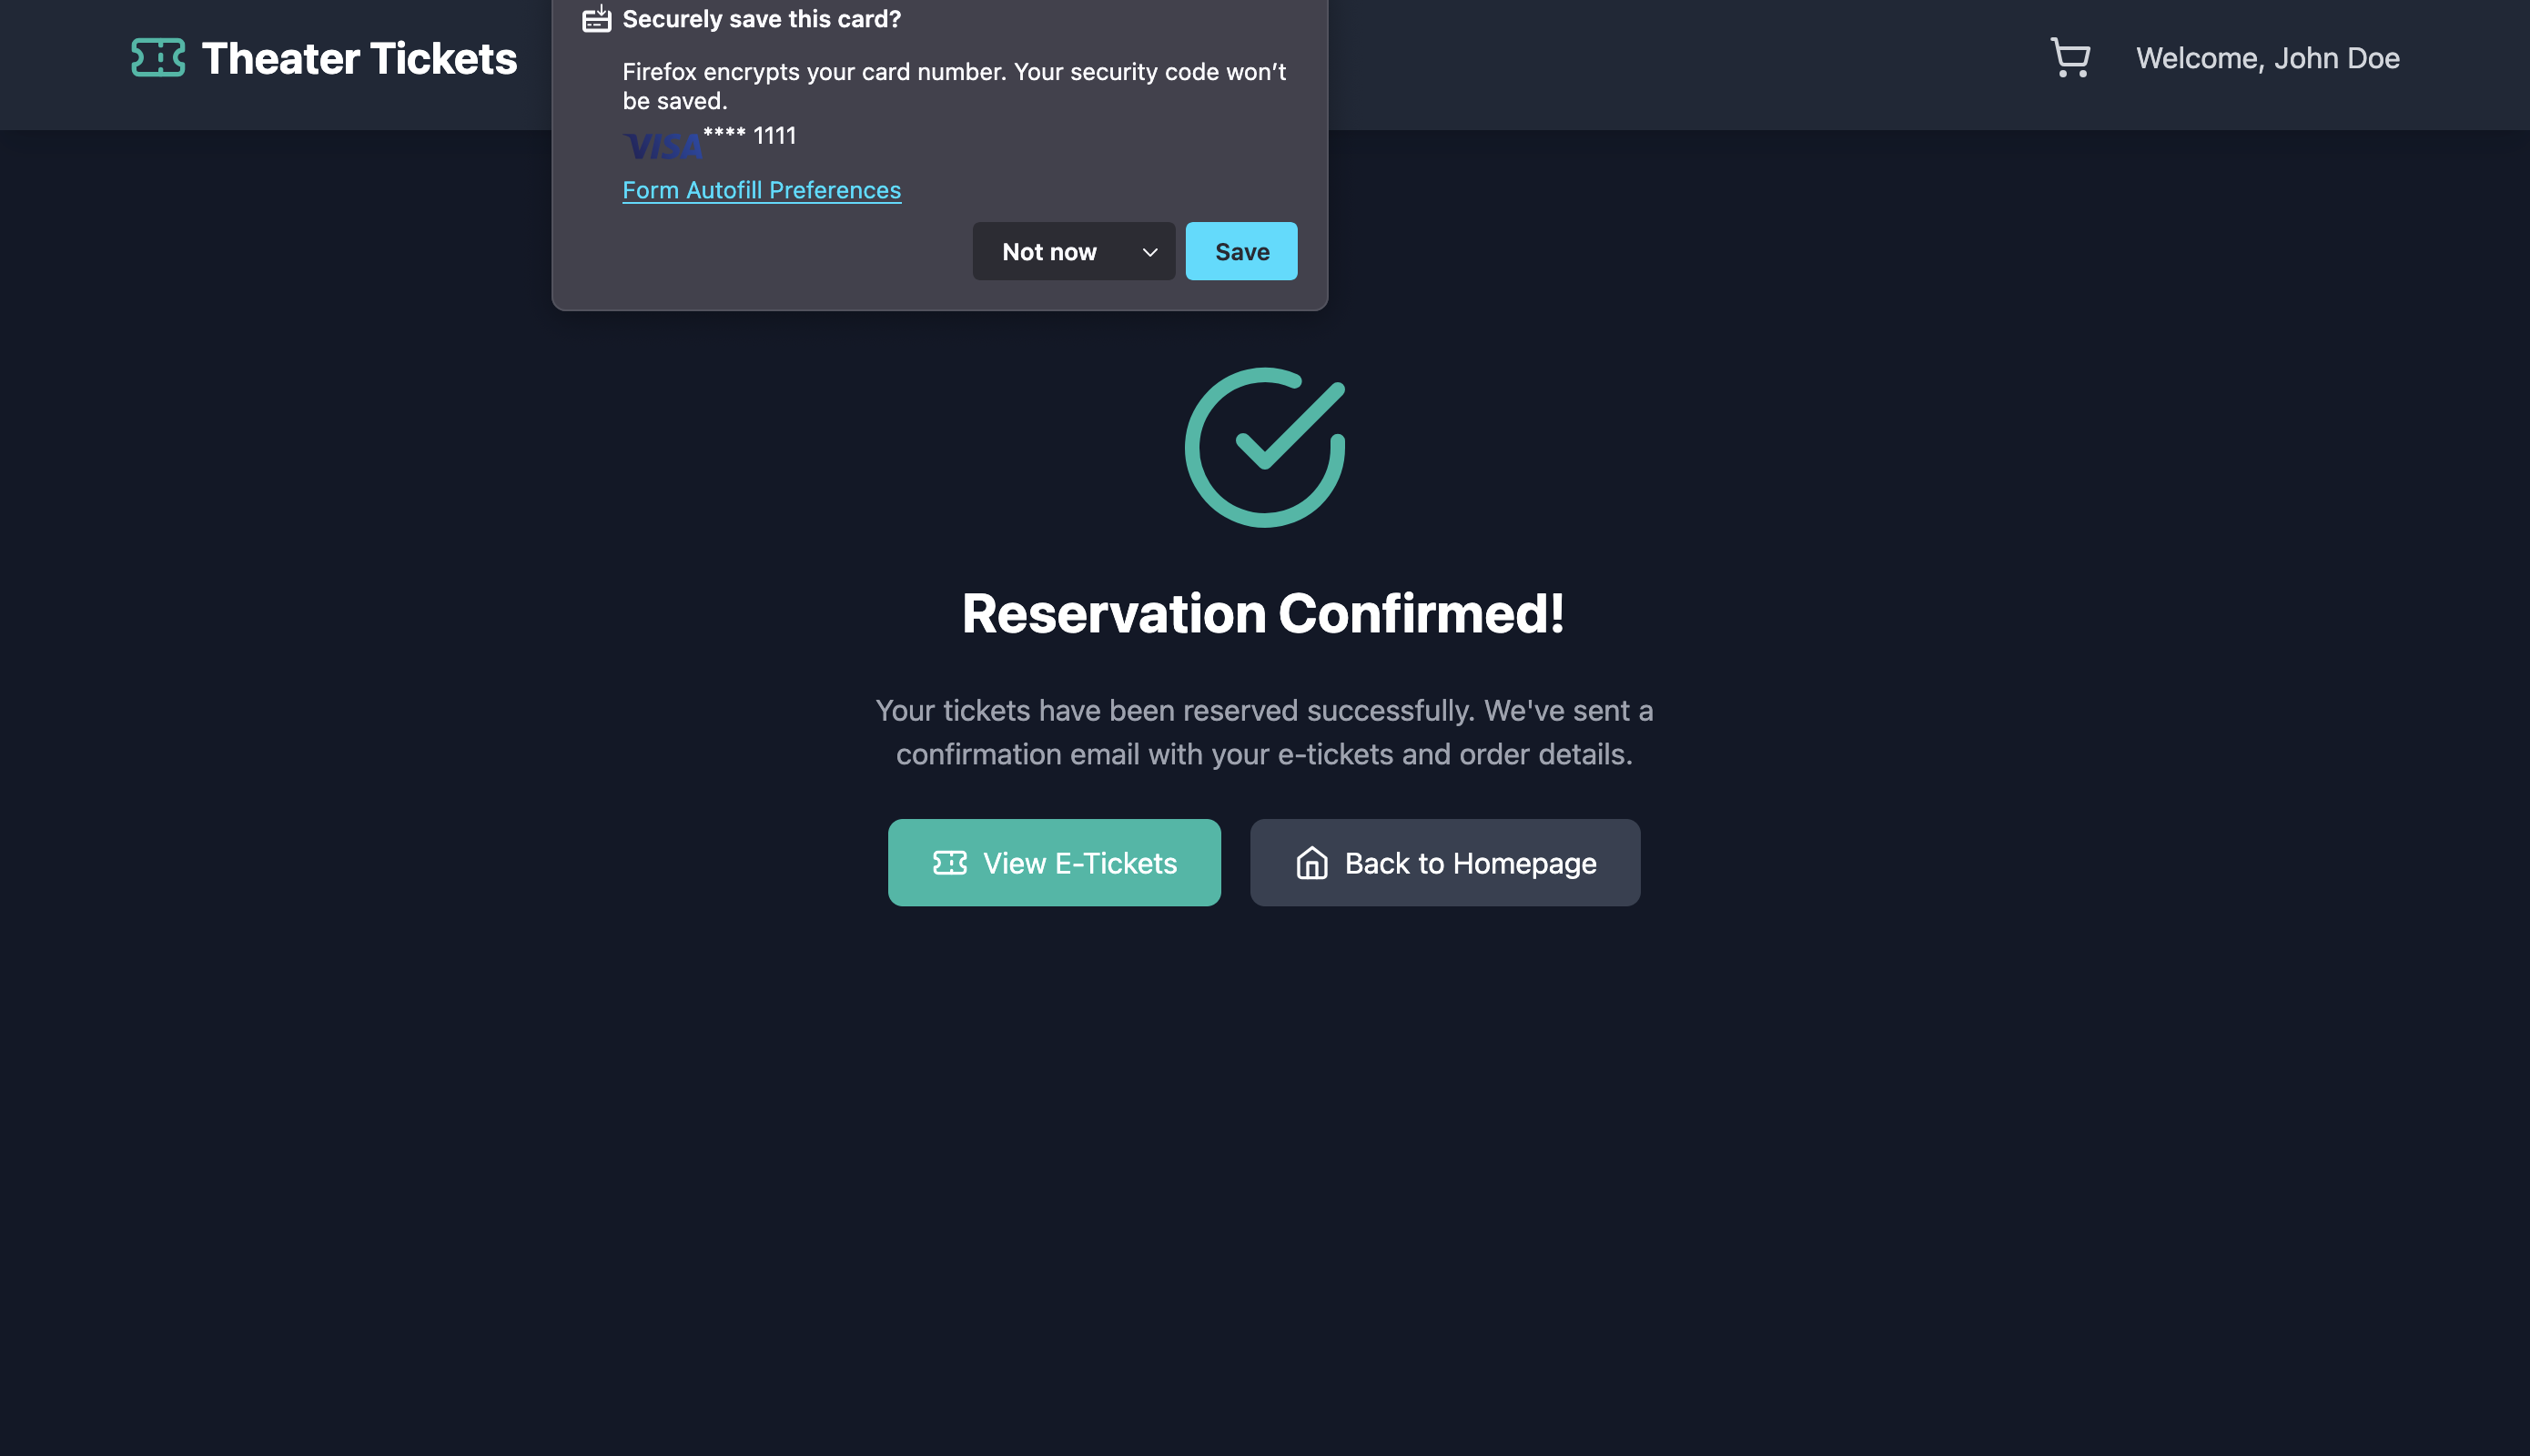
\includegraphics[width=0.9\textwidth]{Slike/FZ2ui/usercomplete.png}
    \caption{Prototip interfejsa za obavijest o uspješnoj registraciji predstave}
    \label{fig:userview}
\end{figure}
\begin{figure}[H]
    \centering
    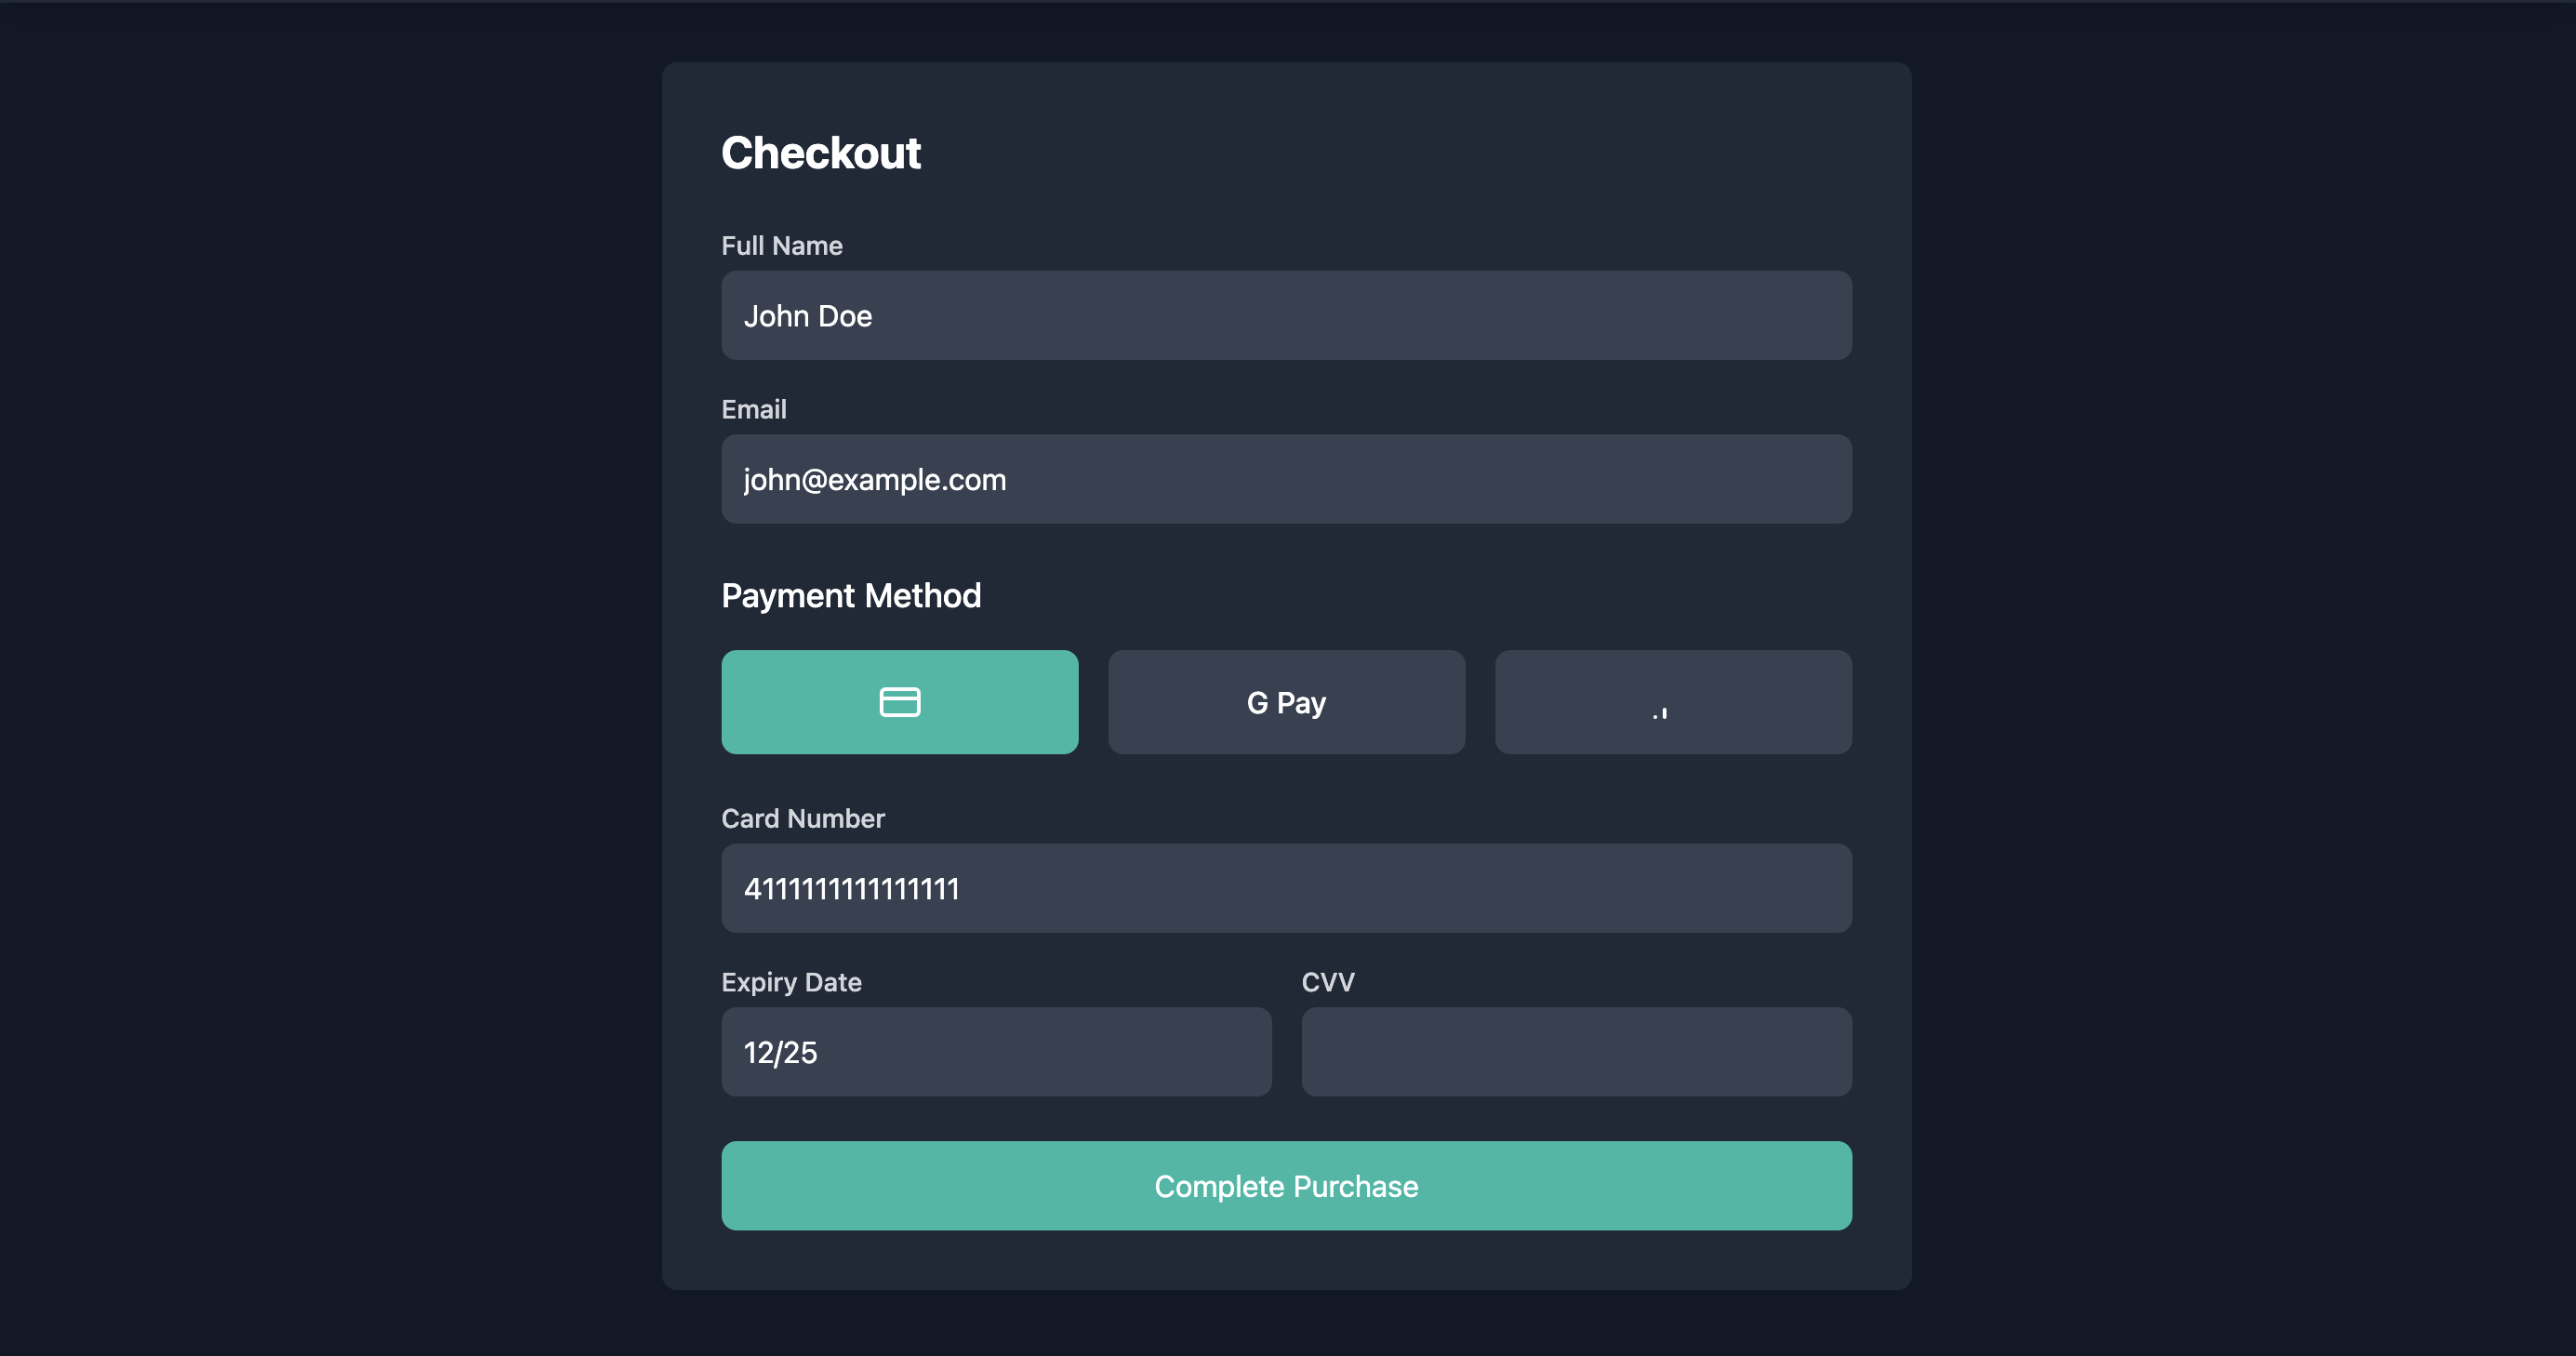
\includegraphics[width=0.9\textwidth]{Slike/FZ2ui/usercheckout.png}
    \caption{Prototip interfejsa za unos podataka o plaćanju za korisnika}
    \label{fig:usercheckout}
\end{figure}
\begin{figure}[H]
    \centering
    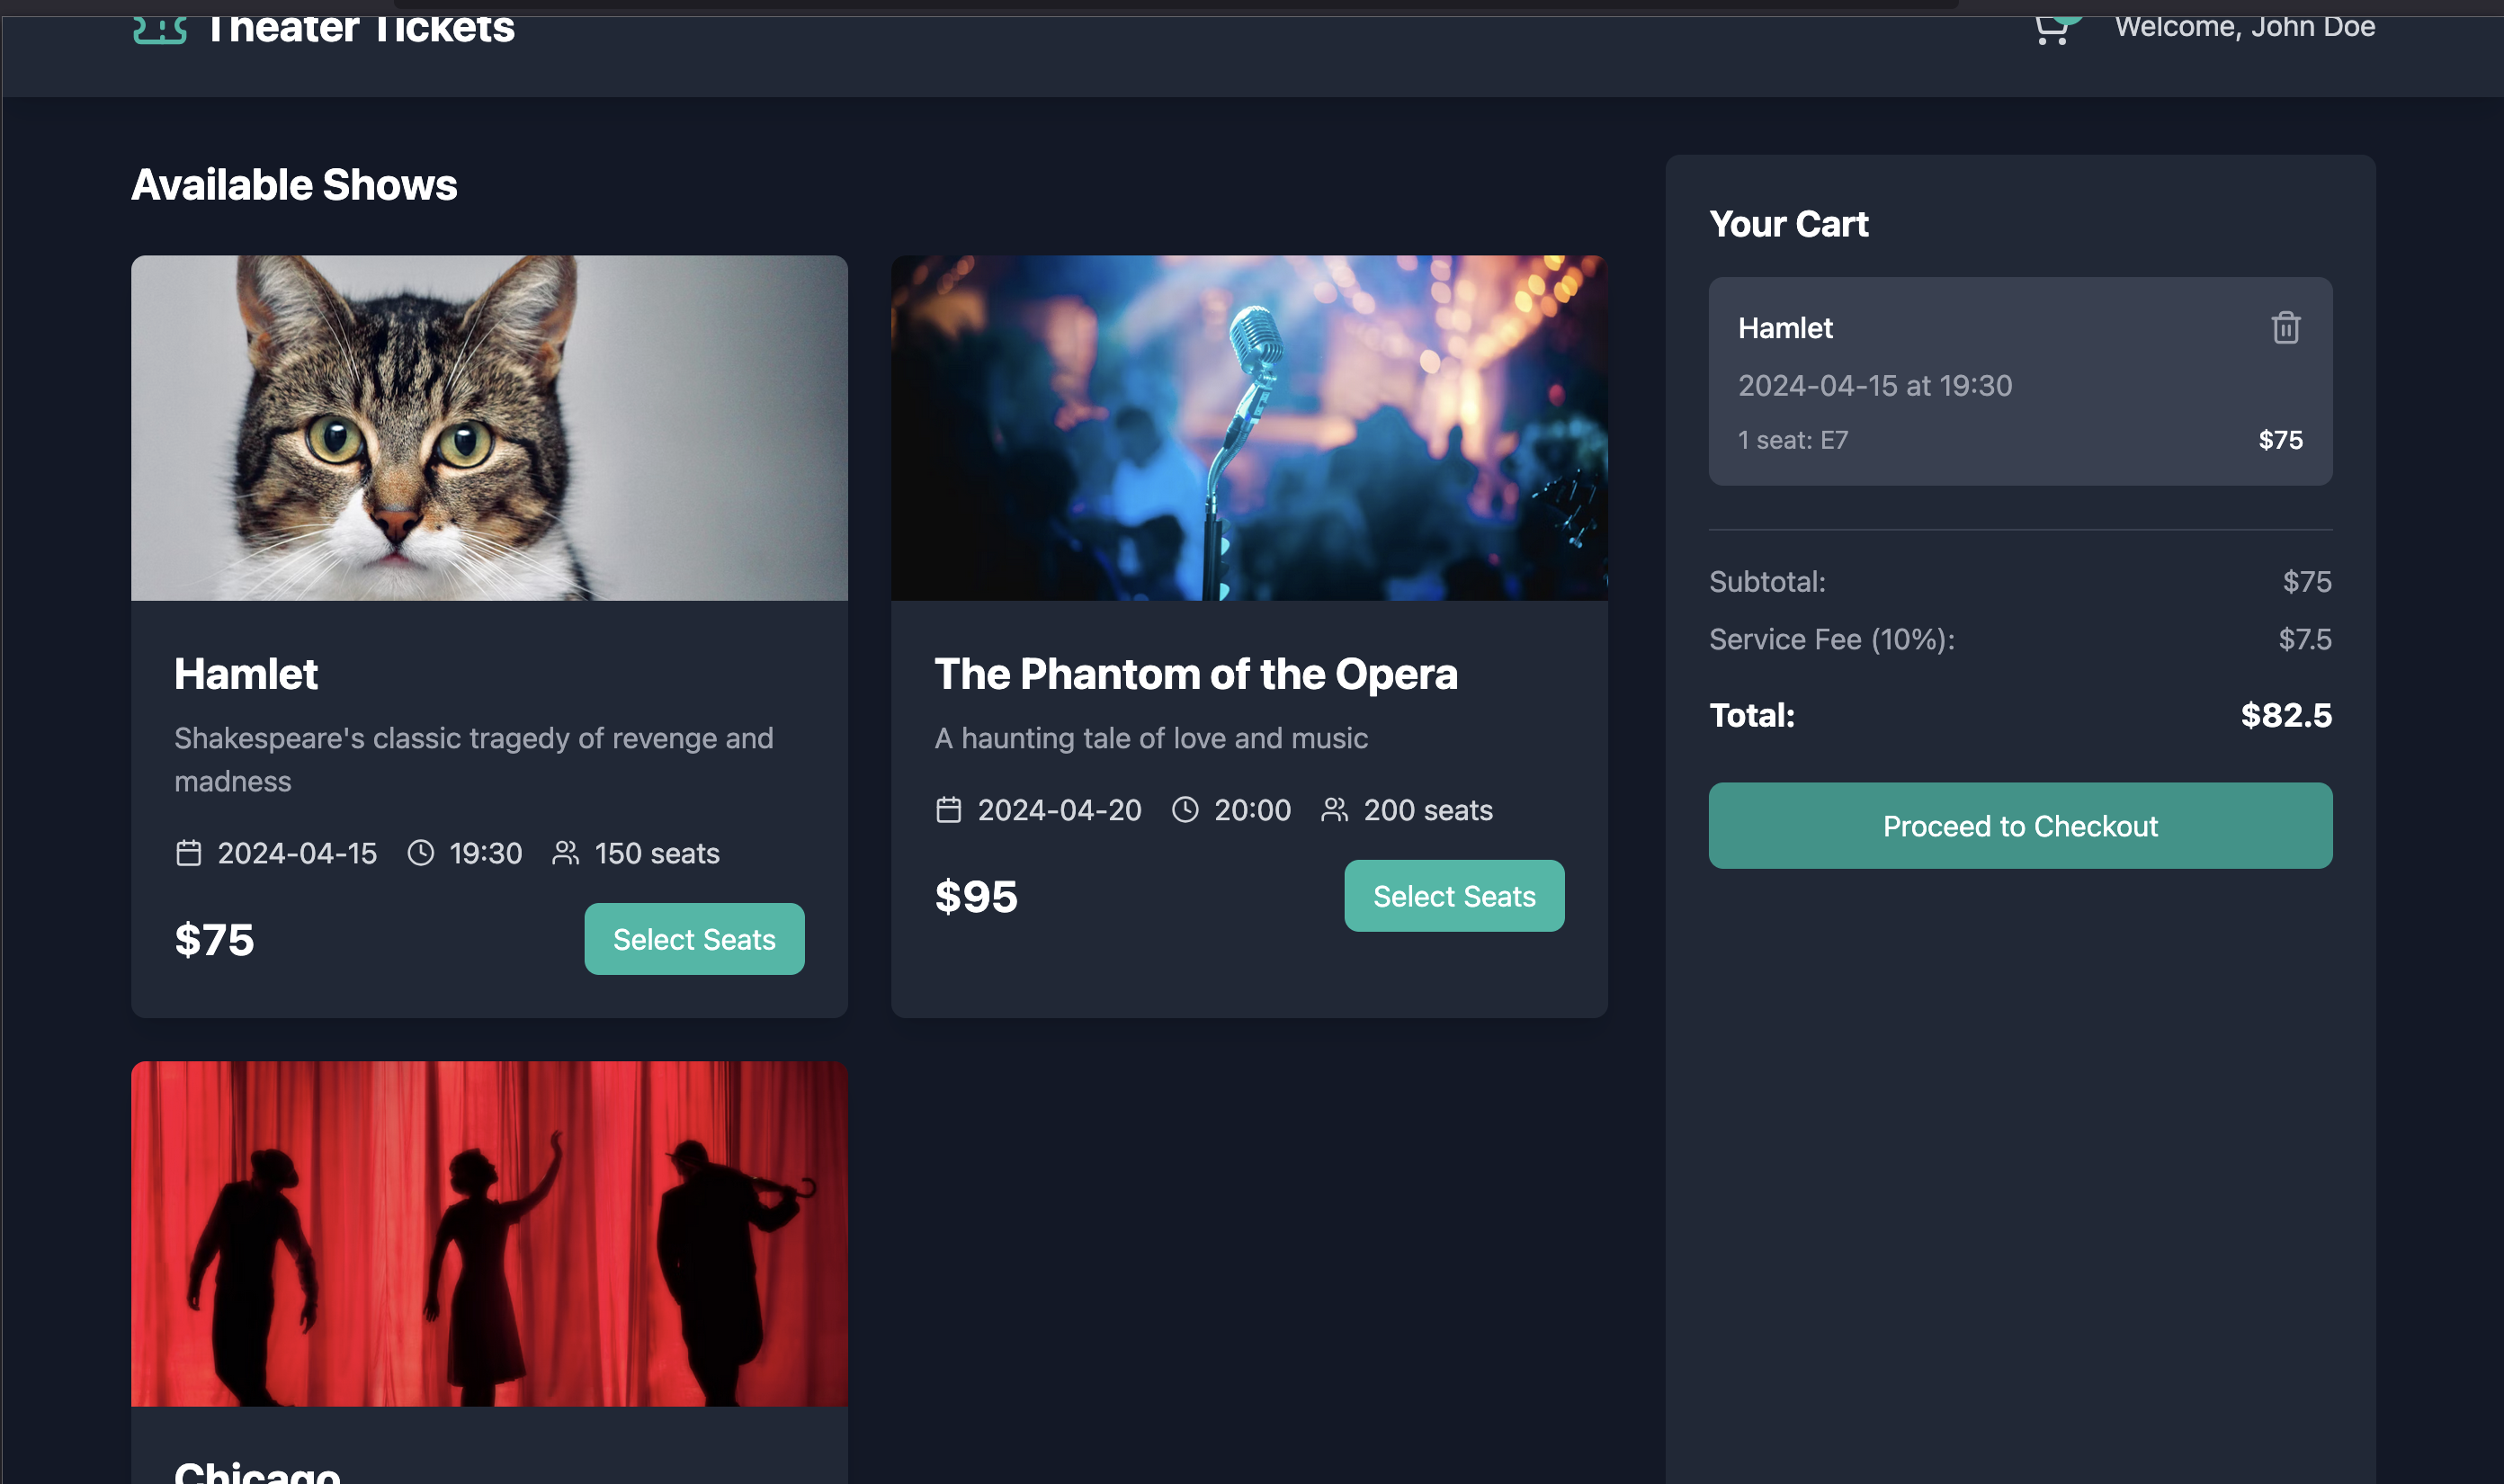
\includegraphics[width=0.9\textwidth]{Slike/FZ2ui/userfrontlist.png}
    \caption{Prototip interfejsa za prikaz korpe}
    \label{fig:userfrontlist}
\end{figure}
\begin{figure}[H]
    \centering
    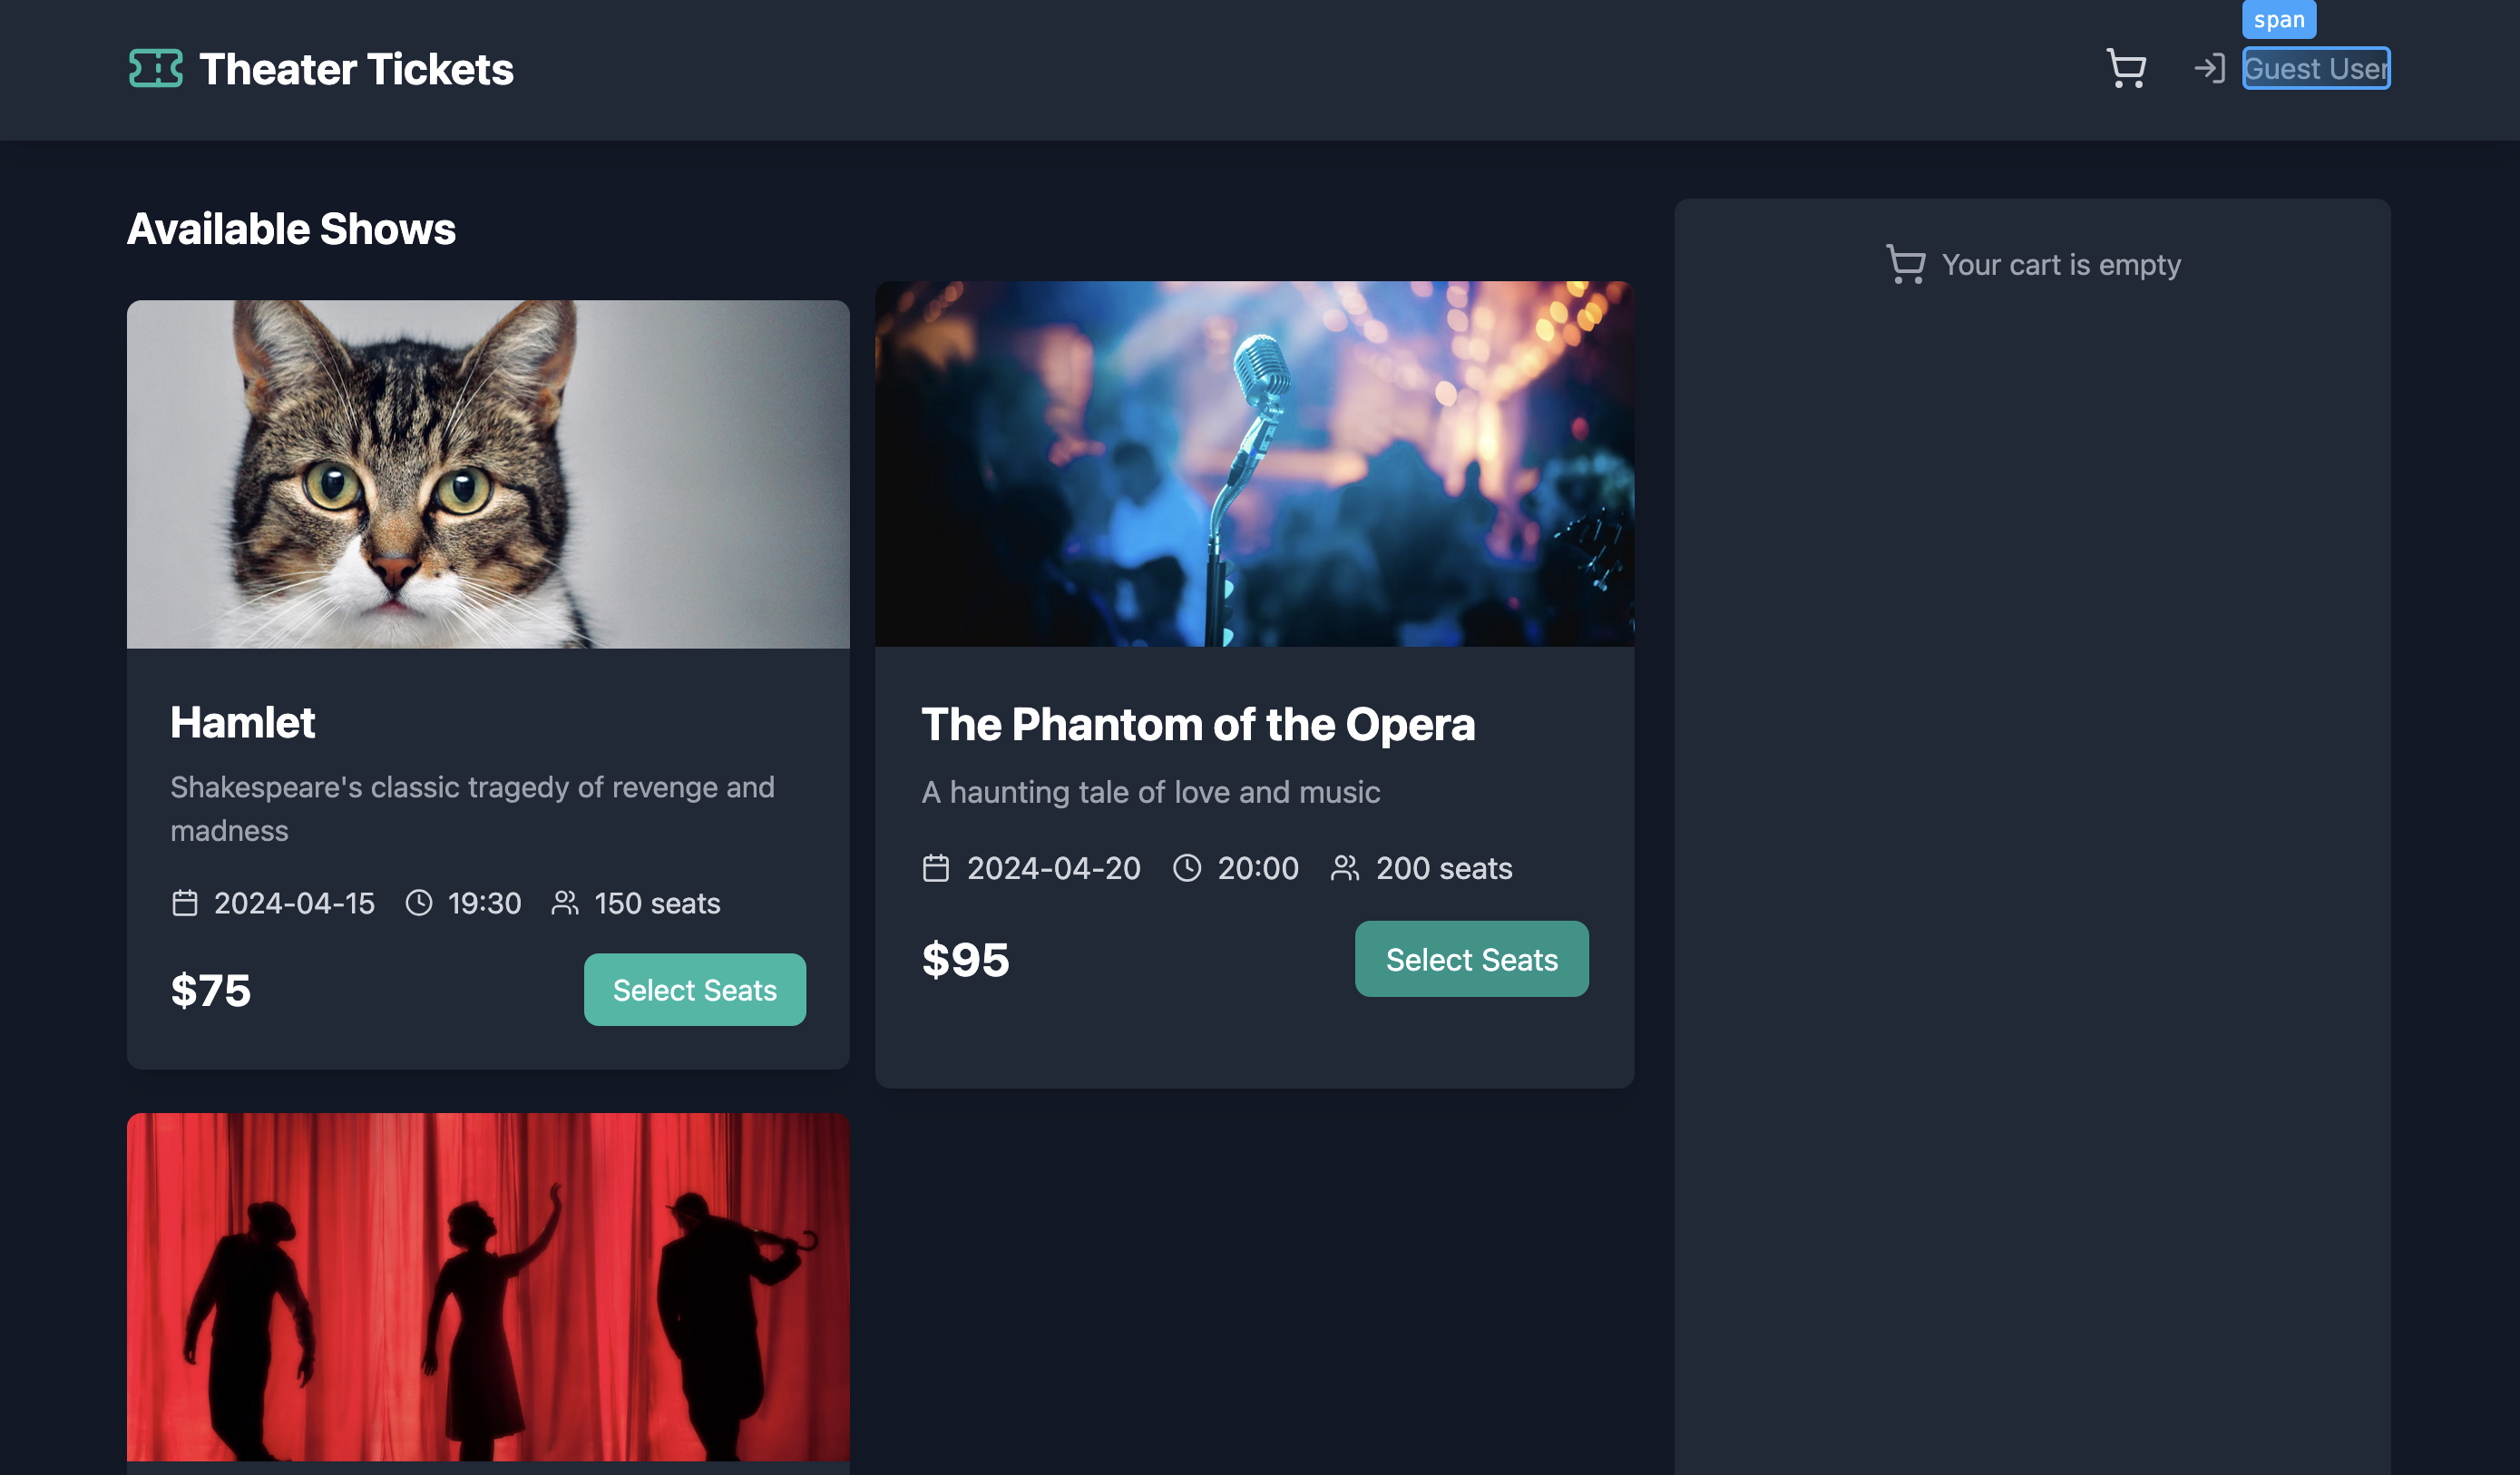
\includegraphics[width=0.9\textwidth]{Slike/FZ2ui/guesthome.png}
    \caption{Prototip interfejsa za prikaz predstava gostu}
    \label{fig:guesthome}
\end{figure}
\begin{figure}[H]
    \centering
    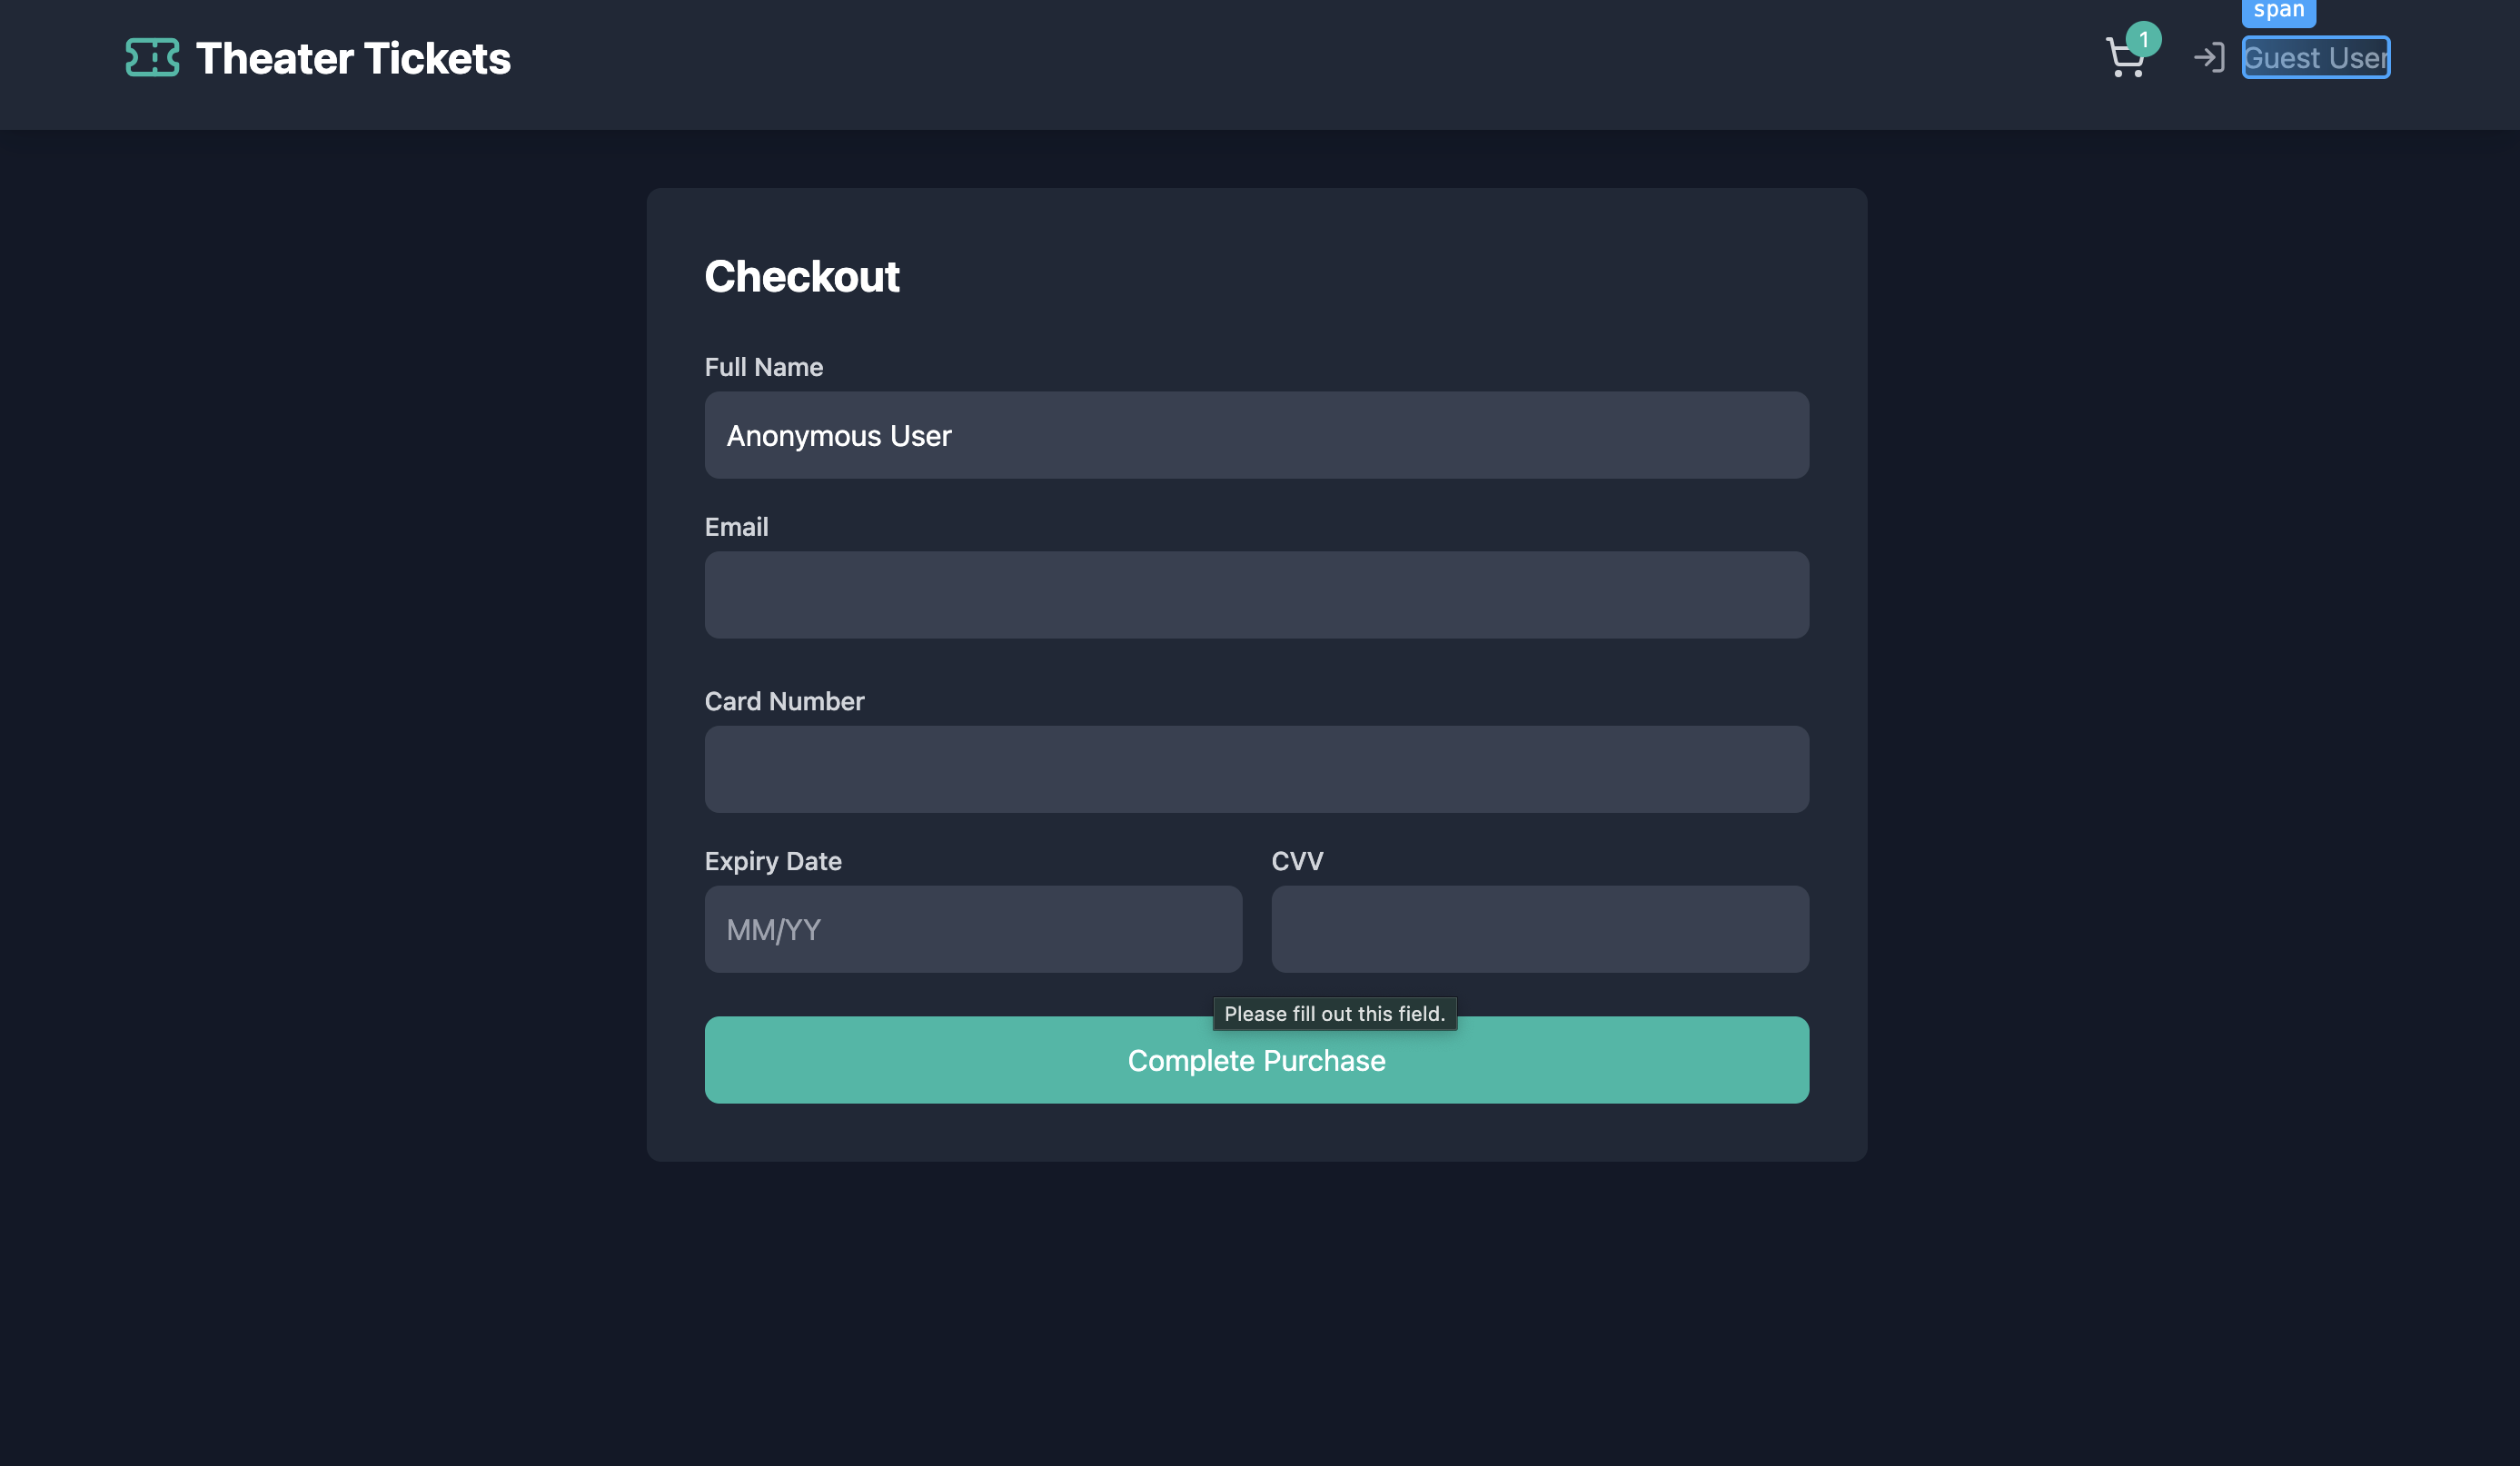
\includegraphics[width=0.9\textwidth]{Slike/FZ2ui/guestcheck.png}
    \caption{Prototip interfejsa za prikaz unosa podataka o plaćanju za neregistrovanog korisnika}
    \label{fig:questcheck}
\end{figure}
\subsection{Bolt promptovi}
\begin{enumerate}[itemsep=1ex]
    \item \textbf{Prvi \textit{prompt}:}

         \textit{ Create a modern and user friendly UI for ticket sales and reservation for a theatre. If the user is not registered he may view active plays, add one to his cart and checkout by filling out a reservation form. A registered user may view active plays, add them to his cart and checkout by choosing a method of payment: Credit Card, Google Pay, PayPal. If the registered user has already made purchases remember them and autofill the checkout. In all cases a message should be displayed for a successful reservation. Make the UI theme in dark mode.}

    \item \textbf{Drugi \textit{prompt}:}

          \begin{enumerate}[itemsep=0.5ex] % Nested list for sub-prompts
              \item Homepage / Play Listing: \textit{Dark mode website homepage UI/UX design for a modern theater ticket sales platform. Features a clean grid layout of cards, each showing a high-quality theater play poster, title, and dates. Prominent call-to-action buttons in teal. Header includes logo, navigation links, cart icon, and login button. Overall professional and user-friendly aesthetic.}  \\

              \item \textit{Play Details \& Seat Selection: \\ Modern dark mode UI/UX screen for theater seat selection. Shows an interactive seat map with a clear stage layout at the top. Seats are displayed in a grid, visually differentiated as available (grey), selected (teal accent color), and unavailable (dark grey/X). A sidebar displays selected seat details and total price. Clean, intuitive web application interface. } \\

           \textit{ Alternative focus: Close-up on an interactive theater seat selection map UI element. Dark mode aesthetic, stage diagram at top, seats clearly marked as available, selected (teal highlight), and booked. Price calculation visible nearby. Modern web design.}  \\

              \item \textit{Shopping Cart:\\ Dark mode shopping cart page UI/UX design for a theater ticket website. Displays a list of selected tickets, showing play title, date, time, seat numbers, quantity, and price per item. Each item has a 'Remove' option. Includes an order summary section calculating subtotal, fees, and total. A clear 'Proceed to Checkout' button uses a teal accent color. Clean and organized layout.} \\

              \item \textit{ Checkout - Unregistered User: \\Modern dark mode checkout screen UI/UX for an unregistered user on a theater ticket website. Features a simple reservation form with fields for Full Name, Email, and Phone Number. A clear order summary is visible (perhaps in a sidebar). A prominent 'Confirm Reservation' button  uses a teal accent color. Minimalist and focused design.} \\

        \item \textit{Checkout - Registered User:\\ Modern dark mode checkout screen UI/UX for a registered user on a theater ticket website. Displays pre-filled user information (Name, Email). Features payment method selection with options for Credit Card (showing input fields for number, expiry, CVV), Google Pay (logo button), and PayPal (logo button). Order summary is clearly visible. A 'Pay Now' button uses a teal accent color. Professional and secure appearance.} \\
                   \textit{ Alternative focus: \\UI/UX detail view of payment method selection on a dark mode checkout page. Shows radio buttons or distinct sections for Credit Card (with masked input fields), Google Pay logo, and PayPal logo. Teal accent color highlights selected option or buttons. Modern web interface.} \\

          \item Success Confirmation: \\Dark mode success confirmation page UI/UX for a theater ticket purchase. Features a large, prominent checkmark icon in a teal accent color. A bold headline reads 'Reservation Confirmed!'. Includes a brief confirmation message mentioning email confirmation and order details recap. Buttons for 'View E-Tickets' or 'Back to Homepage'. Clean, positive, reassuring design. \\
          \end{enumerate}

    \item \textbf{Treći \textit{prompt}:}\\

          \textit{Nithung you generated worked, can you re-do the design so you incorporate funcionalities as well?} % Corrected typo \texit -> \textit
\end{enumerate}

\end{itemize}  

\sloppy  
\newpage
\section{FZ3: Korisnički profil}

\sloppy

\subsection{Opis funkcionalnog zahtjeva}

\begin{itemize}
    \item \textbf{Poslovni proces}: Korisnički profil.
    \item \textbf{Vrste korisnika}: Registrovani korisnik, Administrator.
    \item \textbf{Scenariji korištenja}:
    \begin{enumerate}
        \item \textbf{Registracija novog korisnika}: \\
        Korisnik unosi svoje podatke (ime, prezime, e-mail, lozinka) u registracijski obrazac. Sistem provodi validaciju podataka i šalje verifikacijski e-mail korisniku. Nakon potvrde e-maila, korisnički račun se aktivira.
        
        \item \textbf{Ažuriranje korisničkog profila}: \\
        Registrovani korisnik pristupa svom profilu putem stranice "Moj profil", gdje može ažurirati svoje osobne podatke, dodati ili promijeniti profilnu sliku te pregledati svoju povijest rezervacija i lojalne bodove.
        
        \item \textbf{Administratorski nadzor}: \\
        Administrator ima pristup svim korisničkim profilima i može uređivati ili brisati korisničke račune prema potrebi, uz poštivanje sigurnosnih i privatnih smjernica.
    \end{enumerate}
    \item \textbf{UML dijagram aktivnosti}: Prikazani na slikama \ref{fig:fz3.1} i \ref{fig:fz3.2}
\end{itemize}

\begin{figure}[H]
    \centering
    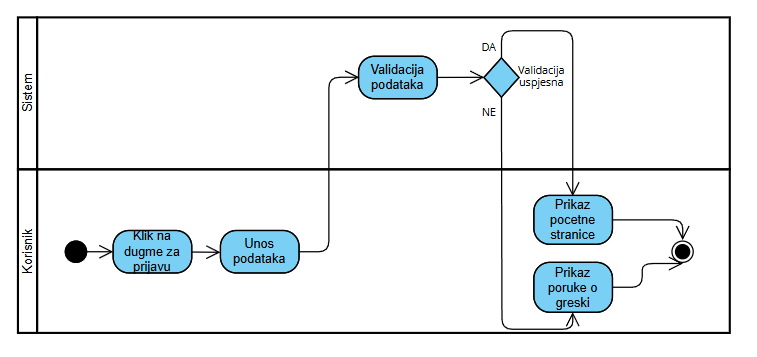
\includegraphics[width=0.9\textwidth]{Slike/fz3.1.png}
    \caption{UML dijagram aktivnosti "Korisnički profil"}
    \label{fig:fz3.1}
\end{figure}

\begin{figure}[H]
    \centering
    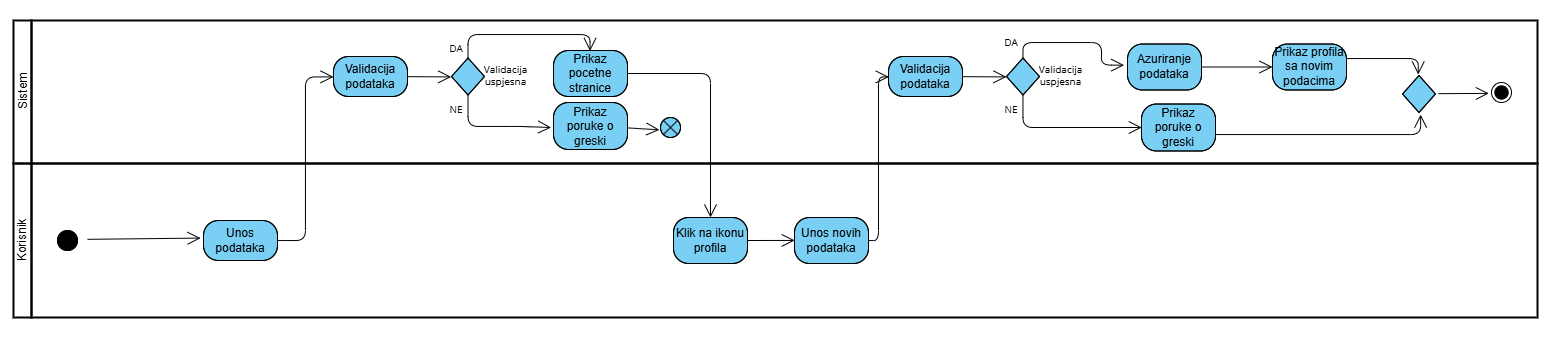
\includegraphics[width=0.9\textwidth]{Slike/fz3.2.png}
    \caption{UML dijagram aktivnosti "Uređivanje Korisničkog profila"}
    \label{fig:fz3.2}
\end{figure}

\sloppy

\subsection{Dizajn korisničkih interfejsa}

\begin{itemize}
    \item \textbf{Prototip interfejsa}: Stranica za registraciju i prijavu, te stranica "Moj profil" s pregledom i uređivanjem korisničkih podataka. Demonstracija ovih funkcionalnosti je prikazana na slikama: \ref{fig:fz3.3}, \ref{fig:fz3.4}, \ref{fig:fz3.5}, \ref{fig:fz3.6}, \ref{fig:fz3.7}, \ref{fig:fz3.8}, \ref{fig:fz3.9}, \ref{fig:fz3.10}
    \item \textbf{Opis scenarija}:
    \begin{itemize}
        \item \textbf{Registracija korisnika}: \\
        Korisnik pristupa stranici za registraciju, unosi svoje podatke i potvrđuje registraciju. Nakon toga, prima verifikacijski e-mail i aktivira svoj račun.
        
        \item \textbf{Prijava korisnika}: \\
        Korisnik unosi svoje pristupne podatke (e-mail i lozinku) na stranici za prijavu. Ako su podaci ispravni, pristupa svom korisničkom profilu.
        
        \item \textbf{Ažuriranje profila}: \\
        Na stranici "Moj profil", korisnik može pregledati i ažurirati svoje osobne podatke, dodati profilnu sliku i pregledati svoju povijest aktivnosti.
    \end{itemize}
\end{itemize}

\begin{figure}[H]
    \centering
    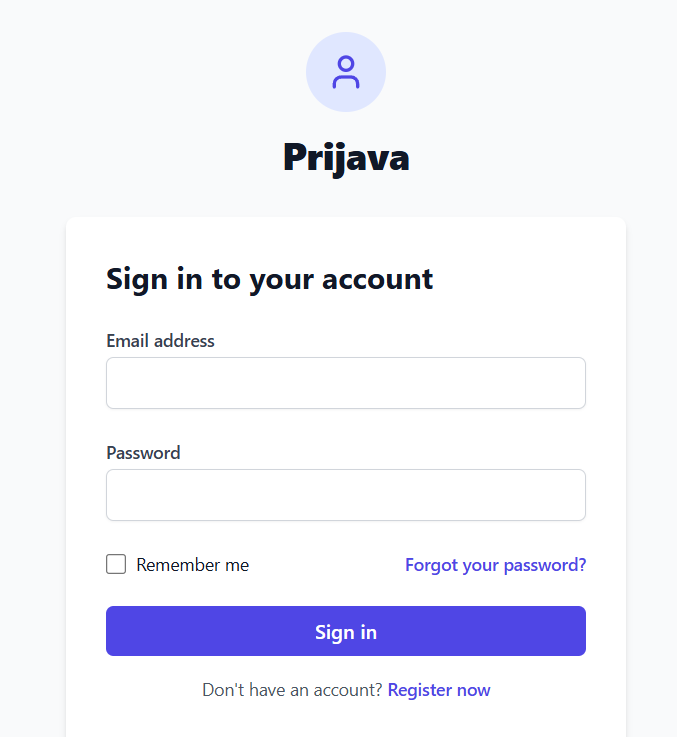
\includegraphics[width=0.9\textwidth]{Slike/fz3.3.png}
    \caption{Prototip stranice za prijavu korisnika}
    \label{fig:fz3.3}
\end{figure}

\begin{figure}[H]
    \centering
    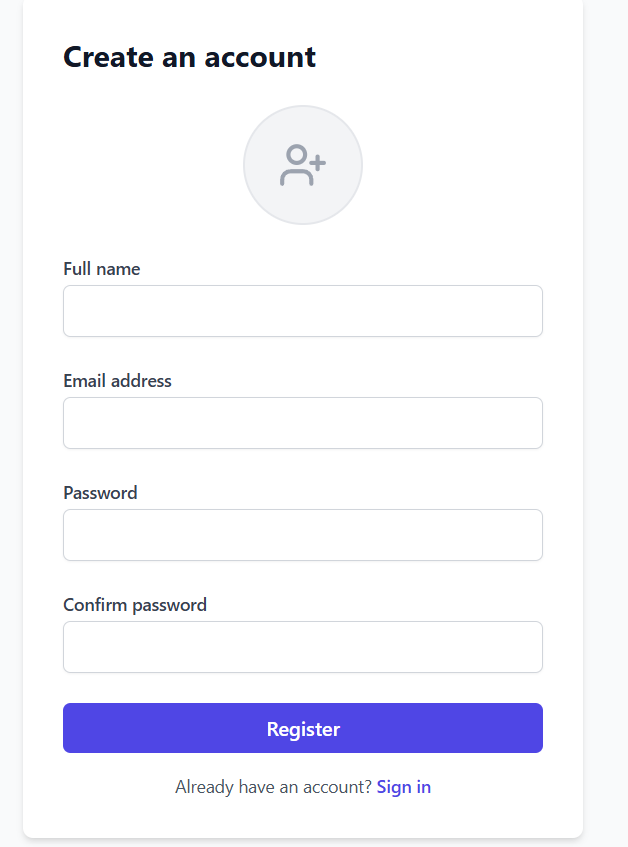
\includegraphics[width=0.9\textwidth]{Slike/fz3.4.png}
    \caption{Prototip stranice za registraciju korisnika}
    \label{fig:fz3.4}
\end{figure}

\begin{figure}[H]
    \centering
    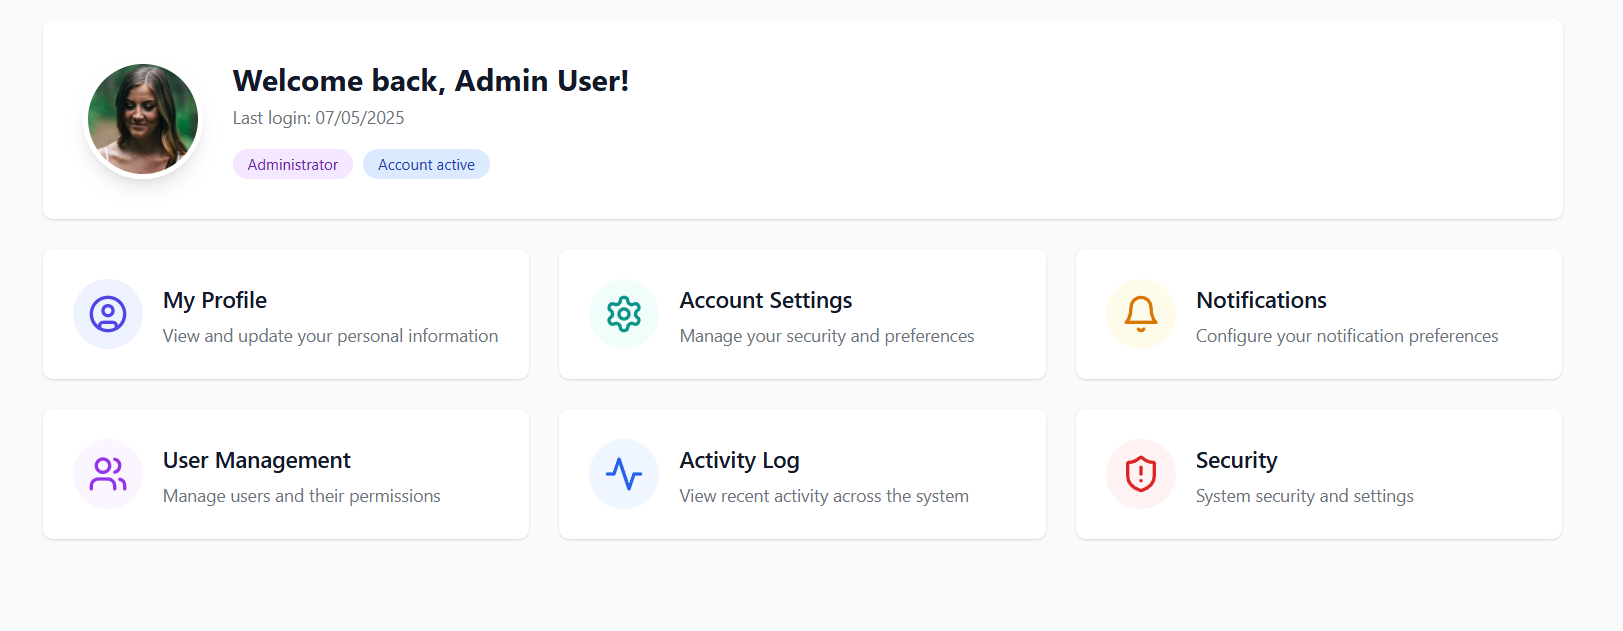
\includegraphics[width=0.9\textwidth]{Slike/fz3.5.png}
    \caption{Admin \textit{dashboard}}
    \label{fig:fz3.5}
\end{figure}

\begin{figure}[H]
    \centering
    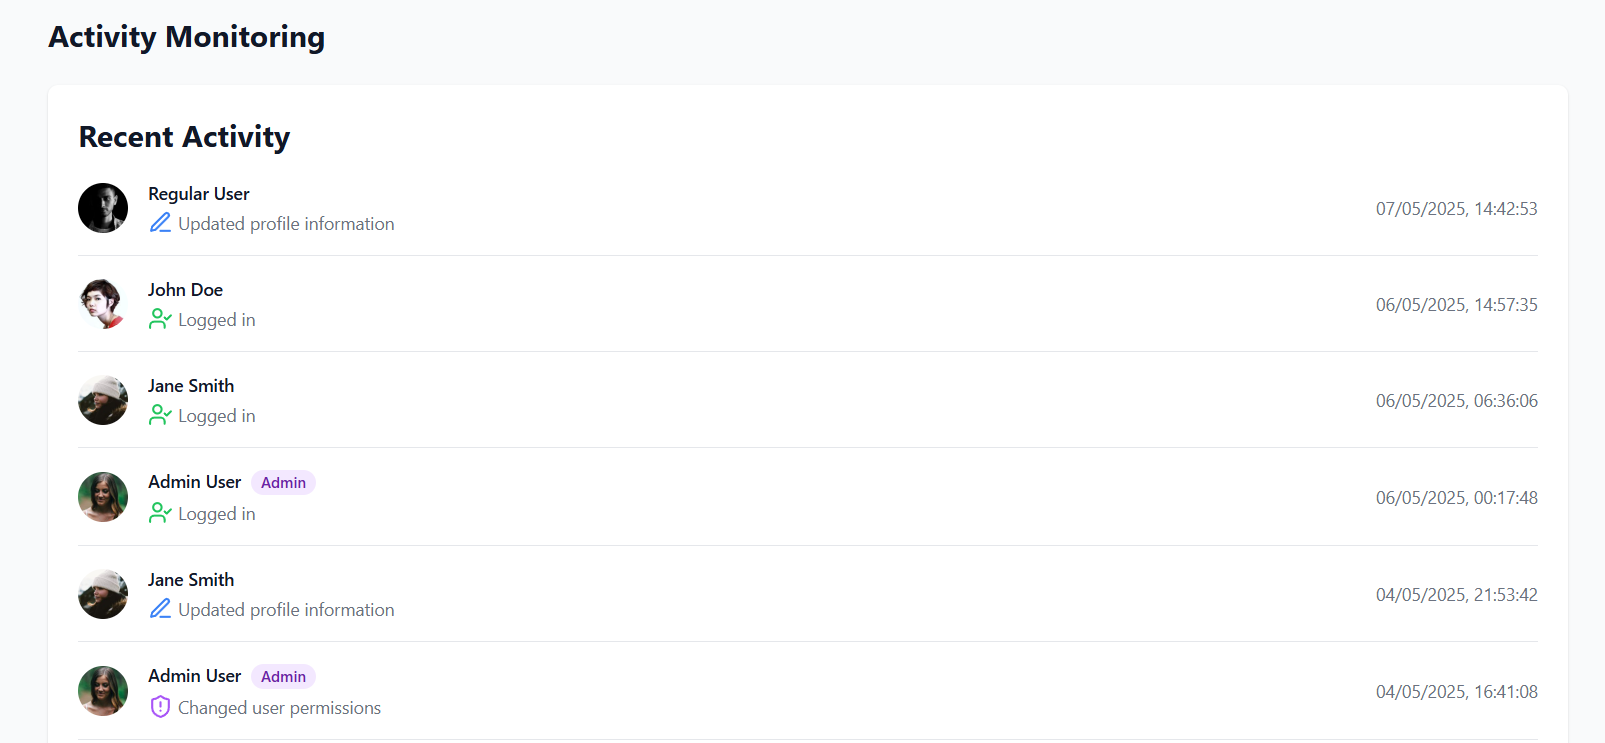
\includegraphics[width=0.9\textwidth]{Slike/fz3.6.png}
    \caption{Pregled aktivnosti korisnika}
    \label{fig:fz3.6}
\end{figure}

\begin{figure}[H]
    \centering
    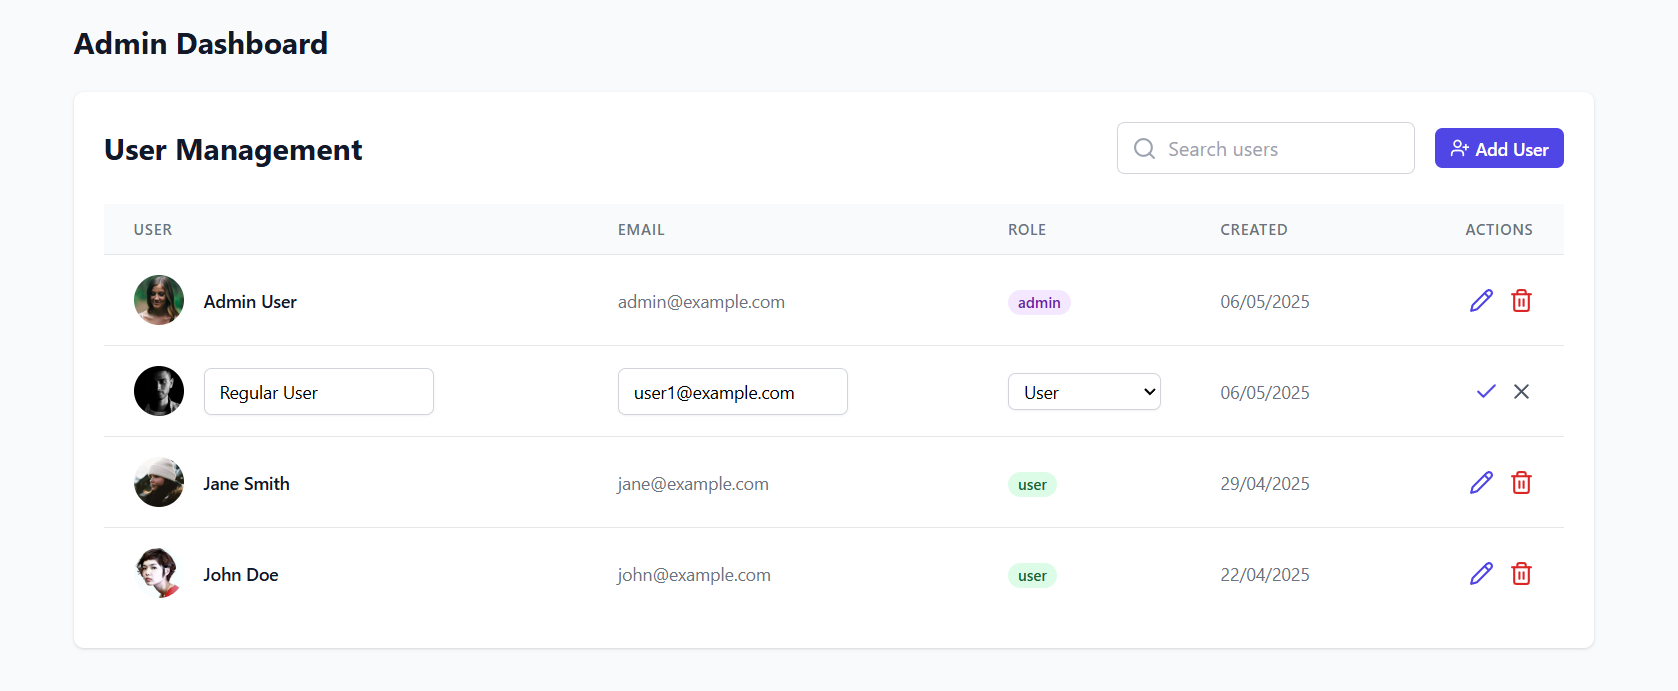
\includegraphics[width=0.9\textwidth]{Slike/fz3.7.png}
    \caption{Pregled svih korisnika i admina}
    \label{fig:fz3.7}
\end{figure}

\begin{figure}[H]
    \centering
    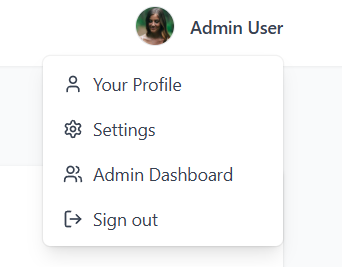
\includegraphics[width=0.9\textwidth]{Slike/fz3.8.png}
    \caption{Opcije dostupne adminima (korisnici nemaju opciju "Admin Dashboard")}
    \label{fig:fz3.8}
\end{figure}

\begin{figure}[H]
    \centering
    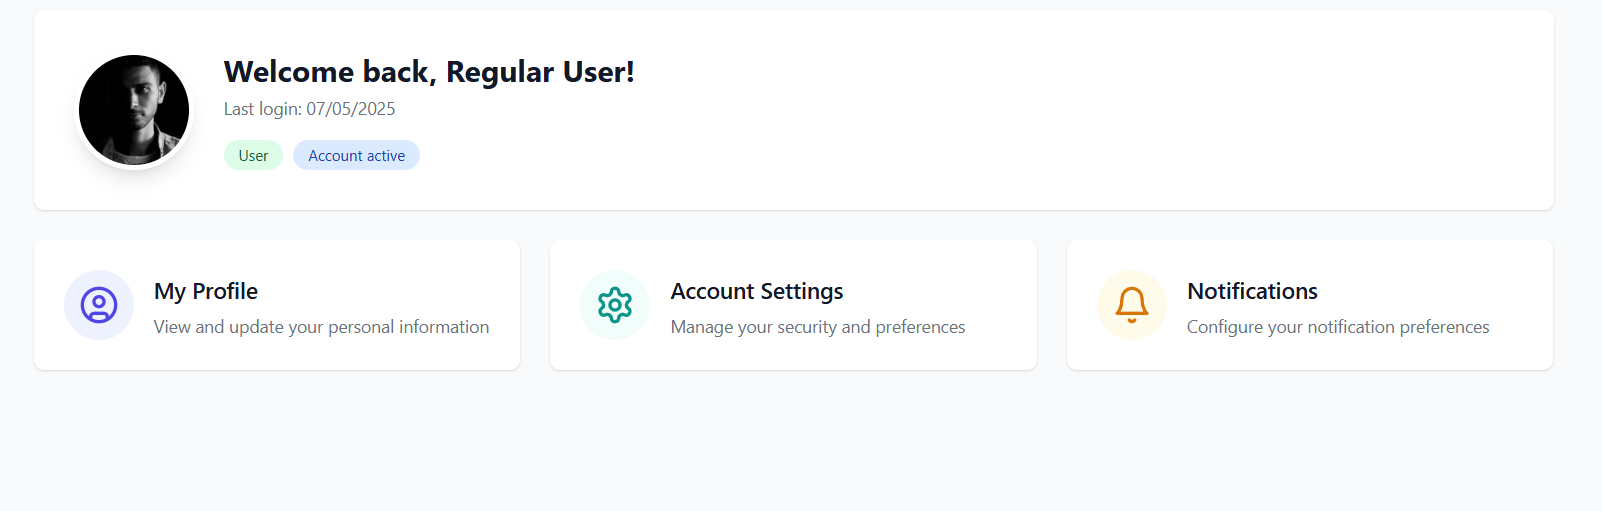
\includegraphics[width=0.9\textwidth]{Slike/fz3.9.png}
    \caption{Prikaz korisnikovog \textit{dashboard}-a}
    \label{fig:fz3.9}
\end{figure}

\begin{figure}[H]
    \centering
    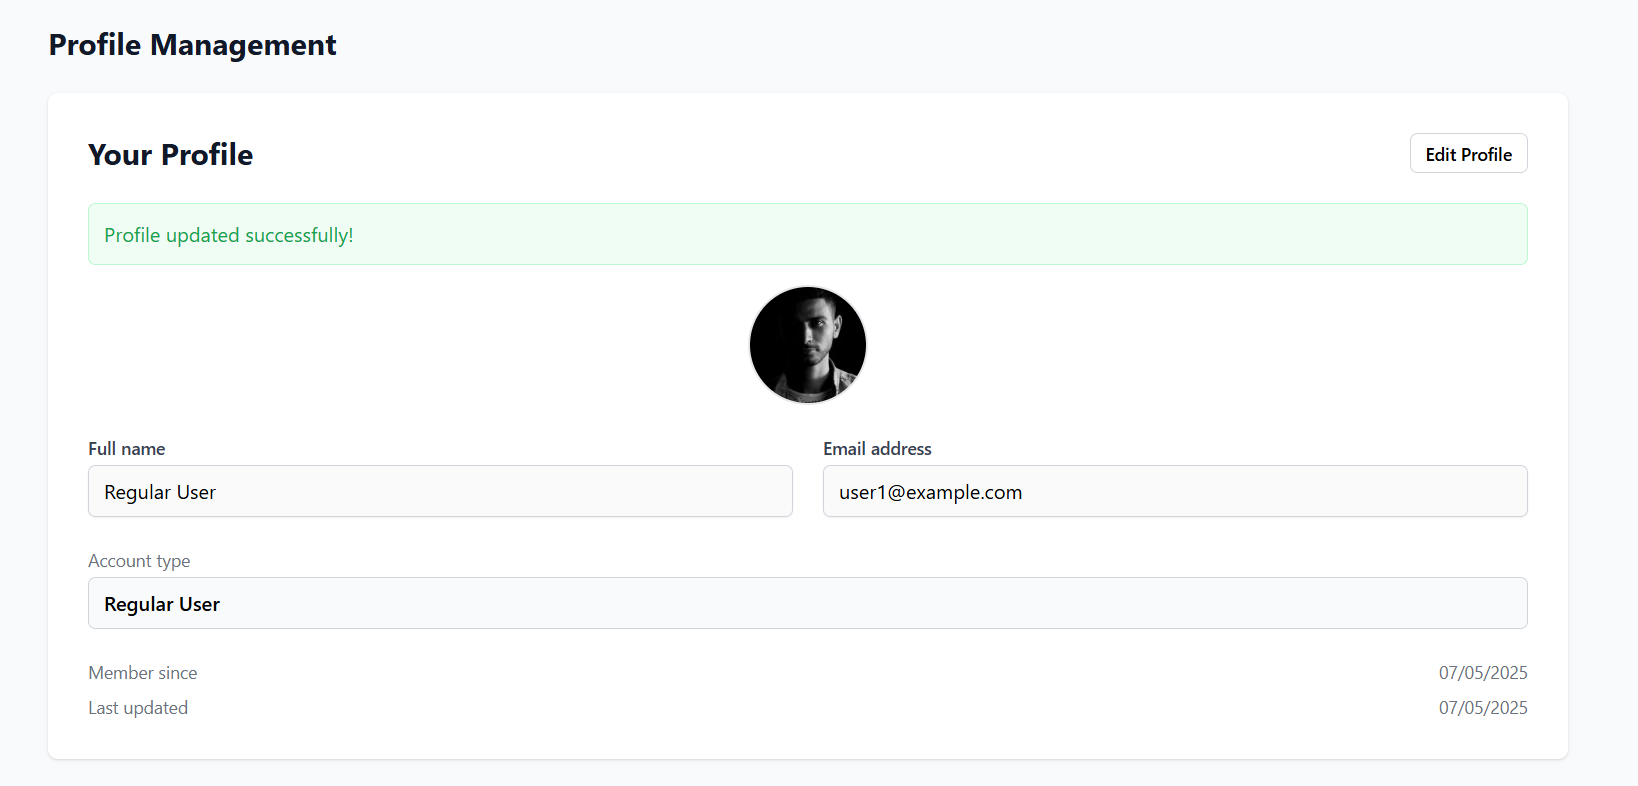
\includegraphics[width=0.9\textwidth]{Slike/fz3.10.png}
    \caption{Uređivanje profila}
    \label{fig:fz3.10}
\end{figure}

\subsection{Bolt \textit{prompt}-ovi}

\begin{enumerate}[itemsep=1ex]
    \item \textbf{Prvi \textit{prompt}:}

         \textit{Objective: Implement a comprehensive user profile management system that allows users to register, update, and manage their profiles, with administrative oversight.Functional Requirements:User Registration: Users must be able to create an account by providing necessary details such as name, email, password, and optional profile picture.Profile Updates: Users can update their personal information, including contact details, password, and preferences.Admin Controls: Administrators should have the ability to view, edit, or delete user profiles as necessary.Business Processes:User Registration:User accesses the registration page.User submits required information.System validates input and creates a new user account.Confirmation email sent to the user.Profile Management:User logs in and accesses their profile.User makes desired changes.System validates and saves changes.Confirmation of successful update displayed.Admin Oversight:Admin accesses user management dashboard.Admin views, edits, or deletes user profiles as needed.}
\end{enumerate}

\newpage  
\section{FZ4: Interaktivni forum}

\sloppy

\subsection{Opis funkcionalnog zahtjeva}

\begin{itemize}
    \item \textbf{Poslovni proces}: Interaktivni forum.
    \item \textbf{Vrste korisnika}: Registrovani korisnik, Gost (samo čitanje).
    \item \textbf{Scenariji korištenja}:
    \begin{enumerate}
        \item \textbf{Čitanje komentara i ocjena predstava}: \\
        Gost ili registrovani korisnik može pristupiti forum stranici određene predstave i pregledavati sve prethodne komentare i ocjene koje su drugi korisnici ostavili.
        
        \item \textbf{Objava novog komentara}: \\
        Registrovani korisnik odabire temu predstave na forumu, unosi svoj komentar ili ocjenu, i objavljuje je. Sistem bilježi vrijeme objave i povezuje komentar sa korisničkim nalogom.
    \end{enumerate}
    \item \textbf{UML dijagram aktivnosti}: Prikazan na slici \ref{fig:fz4}
\end{itemize}

\begin{figure}[H]
    \centering
    \includegraphics[width=1\textwidth]{Slike/Fz4.png}
    \caption{UML dijagram aktivnosti "Interaktivni forum"}
    \label{fig:fz4}
\end{figure}

\sloppy

\subsection{Dizajn korisničkih interfejsa}

\begin{itemize}
    \item \textbf{Prototip interfejsa}: Forum stranica sa listom tema za svaku predstavu, pregledom komentara, ocjenama i poljem za unos novog komentara (samo za registrovane korisnike). Prikazi prototipa interaktivnog foruma su dati na slikama: \ref{fig:fz4.3}, \ref{fig:fz4.4} i \ref{fig:fz4.5}
    \item \textbf{Opis scenarija}:
    \begin{itemize}
        \item \textbf{Dodavanje komentara}: \\
        Registrovani korisnik odabire određenu predstavu, pristupa pripadajućoj temi na forumu, unosi komentar ili ocjenu i potvrđuje objavu.
        
        \item \textbf{Pasivno učešće gosta}: \\
        Gost (neprijavljeni korisnik) može pregledavati sve forume i komentare, ali nema mogućnost dodavanja vlastitih komentara niti interakcije sa drugim korisnicima.
    \end{itemize}
\end{itemize}

\begin{figure}[H]
    \centering
    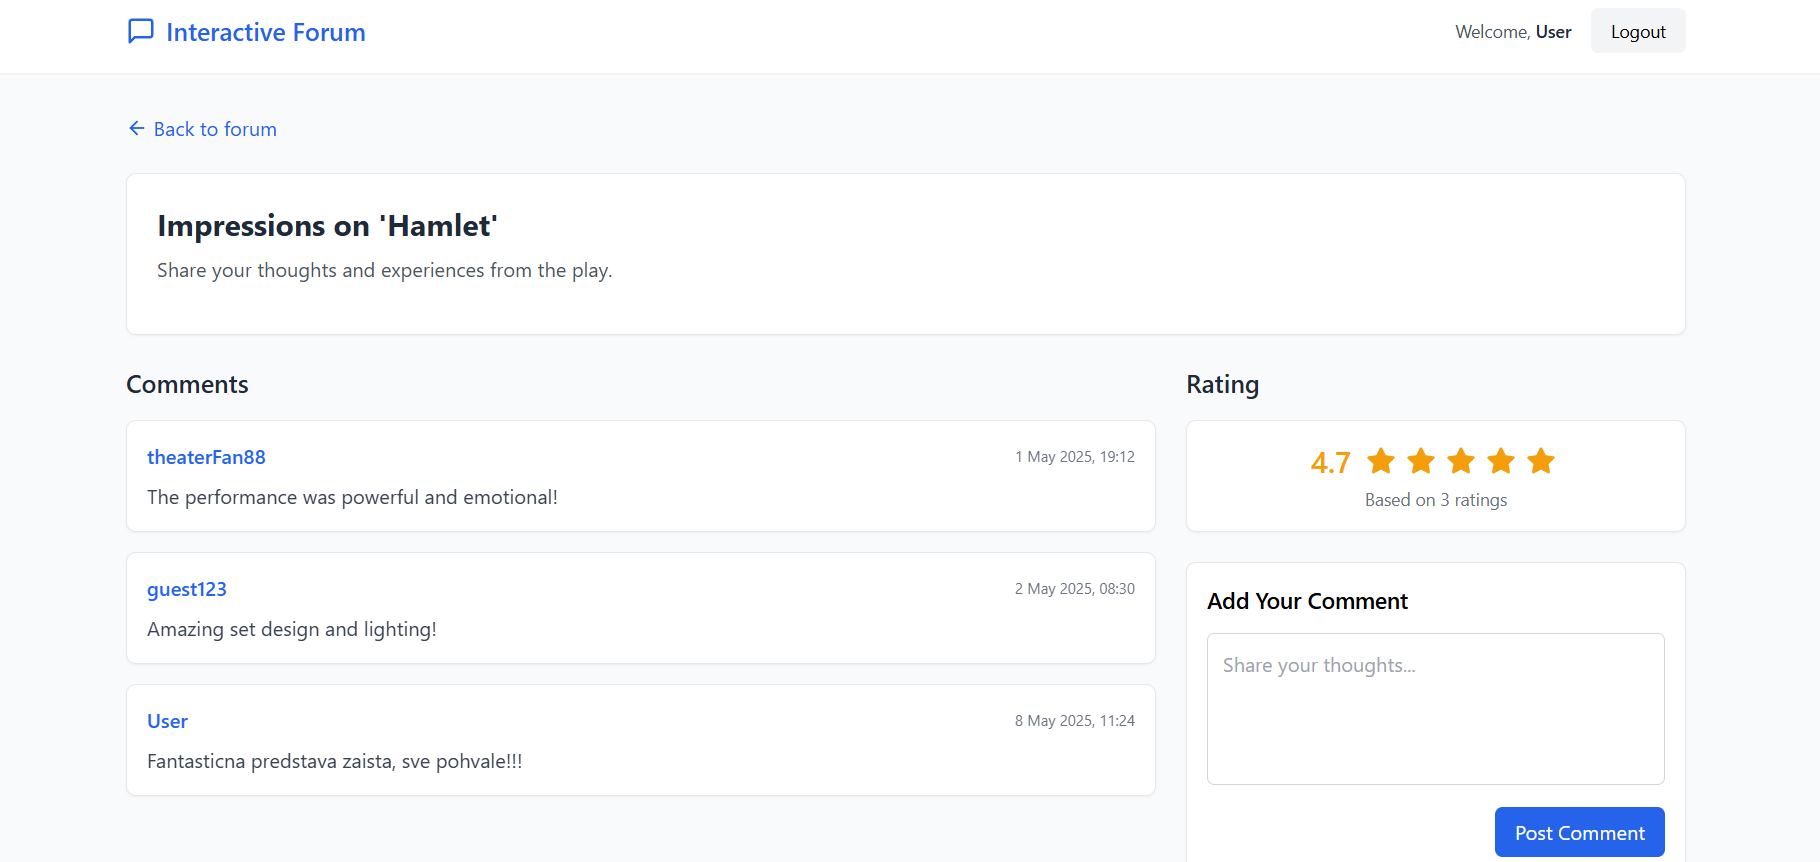
\includegraphics[width=0.9\textwidth]{Slike/fz4.3.png}
    \caption{Prikaz foruma za prijavljenog korisnika i ostavljena recenzija}
    \label{fig:fz4.3}
\end{figure}

\begin{figure}[H]
    \centering
    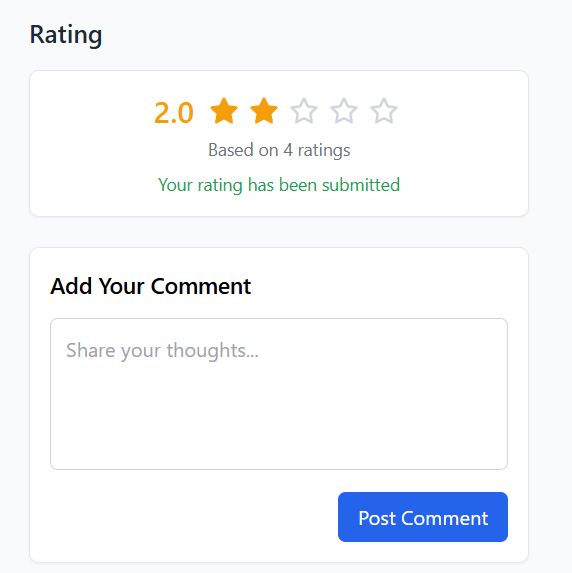
\includegraphics[width=0.9\textwidth]{Slike/fz4.4.png}
    \caption{Ostavljanje ocjene}
    \label{fig:fz4.4}
\end{figure}

\begin{figure}[H]
    \centering
    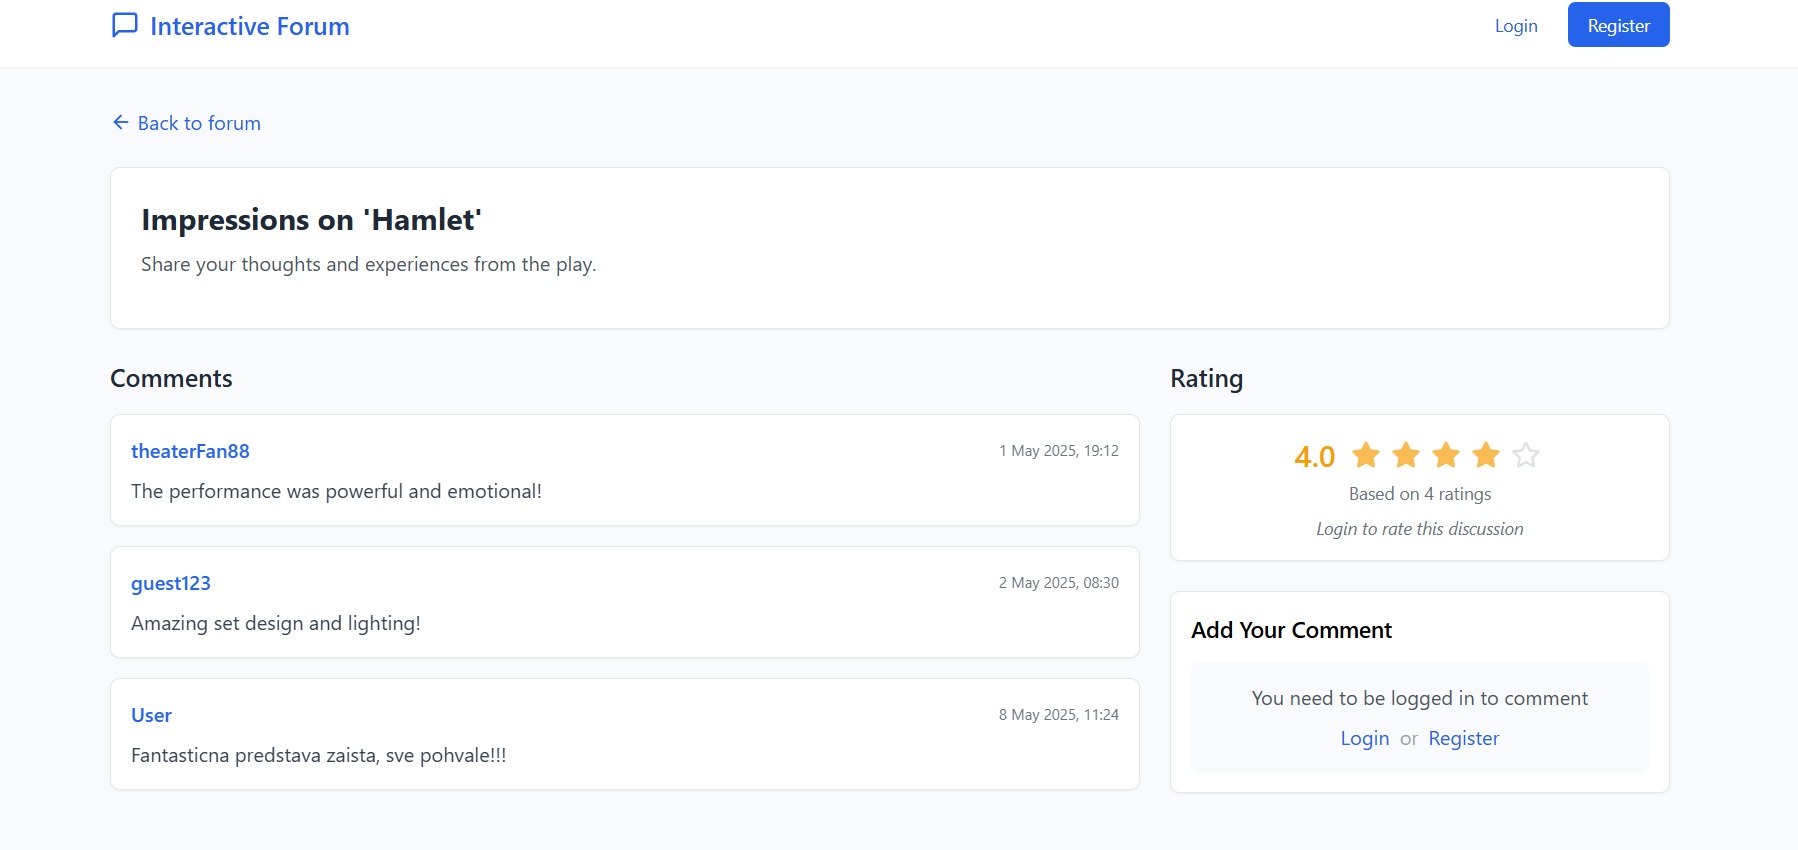
\includegraphics[width=0.9\textwidth]{Slike/fz4.5.png}
    \caption{Prikaz foruma za neprijavljenog korisnika - onemogućeno ostavljanje komentara}
    \label{fig:fz4.5}
\end{figure}

\begin{enumerate}[itemsep=1ex]
    \item \textbf{Prvi \textit{prompt}:}

         \textit{Objective: Develop an interactive forum where users can engage in discussions by posting and commenting, with different access levels for registered users and guests.Functional Requirements:Viewing Discussions: All users, including guests, can read existing forum threads and comments.Posting Comments: Registered users can post new comments in threads.Admin Moderation: Administrators can manage threads and comments, including deletion and reporting.Business Processes:Viewing Discussions:User accesses the forum page.System displays a list of threads with the number of comments.User selects a thread to view detailed comments.Posting Comments:Registered user logs in and selects a thread.User types and submits a comment.System validates and posts the comment.Confirmation of successful post displayed.Admin Moderation:Admin accesses the forum management dashboard.Admin reviews and manages threads and comments.System logs admin actions for auditing purposes.User Types:Registered Users: Can post comments and participate in discussions.Guests: Can only view threads and comments; cannot post.Administrators: Can manage all aspects of the forum.Usage Scenarios:Scenario 1: A guest reads through a discussion thread without posting.Scenario 2: A registered user logs in, posts a comment, and receives confirmation.Scenario 3: An administrator moderates a thread by deleting inappropriate comments.User Interface Design:Forum Page:List of discussion threads with titles and comment counts about theatre plays.Pagination or infinite scroll for thread navigation.Search bar to filter threads by keywords.Thread View:Display of original post and subsequent comments.Input field for registered users to submit new comments."Post Comment" button to submit.Admin options to delete or report comments.}
\end{enumerate}



\sloppy  
\section{FZ5: Integracija društvenih mreža}  

\sloppy  
\subsection{Opis funkcionalnog zahtjeva}  
\begin{itemize}  
    \item \textbf{Poslovni proces}: Kreiranje i uređivanje korisničkih profila.  
    \item \textbf{Vrste korisnika}: Registrovani korisnik, Administrator.  
    \item \textbf{Scenariji korištenja}:  
        \begin{enumerate}  
            \item Dijeljenje predstave na Instagram/TikTok direktno iz platforme.  
            \item Prijava u sistem preko Facebook/Google naloga.  
        \end{enumerate}  
    \item \textbf{UML dijagram aktivnosti}: Prikazan na slici \textbf{SLIKA4}  
\end{itemize}  

\sloppy  
\subsection{Dizajn korisničkih interfejsa}  
\begin{itemize}  
    \item \textbf{Prototip interfejsa}: Dugmad "Podijeli" na stranici predstave i opcija "Prijavi se putem društvene mreže" (slika \textbf{SLIKA4}  
    \item \textbf{Opis scenarija}:  
        \begin{itemize}  
            \item Korisnik klikne na "Podijeli" i odabire platformu za dijeljenje.  
            \item Novi korisnik registruje se preko društvene mreže bez ručnog unosa podataka.  
        \end{itemize}  
\end{itemize}  


\sloppy  
\section{FZ6: Marketing i obavještenja}  

\sloppy  
\subsection{Opis funkcionalnog zahtjeva}  
\begin{itemize}  
    \item \textbf{Poslovni proces}: Online prodaja i rezervacija karata s višestrukim načinima plaćanja 
    \item \textbf{Vrste korisnika}: Administrator, Registrovani korisnik.  
    \item \textbf{Scenariji korištenja}:  
        \begin{enumerate}  
            \item Kreiranje e-mail/SMS kampanje za novu predstavu.  
            \item Pretplata korisnika na newsletter.  
        \end{enumerate}  
    \item \textbf{UML dijagram aktivnosti}: Prikazan na slici \textbf{SLIKA5}  
\end{itemize}  

\sloppy  
\subsection{Dizajn korisničkih interfejsa}  
\begin{itemize}  
    \item \textbf{Prototip interfejsa}: Dashboard za kreiranje kampanja i postavke za notifikacije (slika \textbf{SLIKA5}  
    \item \textbf{Opis scenarija}:  
        \begin{itemize}  
            \item Administrator odabire ciljnu grupu i šalje promotivni e-mail.  
            \item Korisnik prima obavijest o popustu i klikom otvara stranicu za kupovinu.  
        \end{itemize}  
\end{itemize}  

\sloppy  
\section{FZ7: Višekanalna korisnička podrška i komunikacija}  

\sloppy  
\subsection{Opis funkcionalnog zahtjeva}  
\begin{itemize}  
    \item \textbf{Poslovni proces}: Kreiranje i uređivanje korisničkih profila   
    \item \textbf{Vrste korisnika}: Korisnik, Podrška.  
    \item \textbf{Scenariji korištenja}:  
        \begin{enumerate}  
            \item Korisnik postavlja upit putem chatbota.  
            \item Podrška odgovara na e-mail zahtjev.  
        \end{enumerate}  
    \item \textbf{UML dijagram aktivnosti}: Prikazan na slici \textbf{Slika7}  
\end{itemize}  

\sloppy  
\subsection{Dizajn korisničkih interfejsa}  
\begin{itemize}  
    \item \textbf{Prototip interfejsa}: Chat prozor u donjem desnom uglu i stranica za slanje e-maila (slika \textbf{Slika7-ui}).  
    \item \textbf{Opis scenarija}:  
        \begin{itemize}  
            \item Korisnik piše pitanje u chatbot, koji nudi automatske odgovore ili preusmjerava na e-mail.  
            \item Podrška prati sve zahtjeve preko ticketing sistema.  
        \end{itemize}  
\end{itemize}  

\sloppy  
\section{FZ8: Personalizovane notifikacije o novim predstavama i ponudama}  

\sloppy  
\subsection{Opis funkcionalnog zahtjeva}  
\begin{itemize}  
    \item \textbf{Poslovni proces}: Kreiranje i uređivanje korisničkih profila  
    \item \textbf{Vrste korisnika}: Registrovani korisnik, Administrator.  
    \item \textbf{Scenariji korištenja}:  
        \begin{enumerate}  
            \item Slanje automatskih obavijesti o novim predstavama.  
            \item Personalizacija postavki notifikacija (e-mail/SMS).  
        \end{enumerate}  
    \item \textbf{UML dijagram aktivnosti}: Prikazan na slici \textbf{Slika8}  
\end{itemize}  

\sloppy  
\subsection{Dizajn korisničkih interfejsa}  
\begin{itemize}  
    \item \textbf{Prototip interfejsa}: Postavke profila s opcijama za notifikacije i admin panel za slanje masovnih obavijesti (slika \textbf{Slika8-ui}).  
    \item \textbf{Opis scenarija}:  
        \begin{itemize}  
            \item Korisnik odabire želi li primati obavijesti putem e-maila ili SMS-a.  
            \item Administrator šalje promociju za sezonsku ponudu.  
        \end{itemize}  
\end{itemize}  

\sloppy  
\section{FZ9: Moderacija foruma}  

\sloppy  
\subsection{Opis funkcionalnog zahtjeva}  
\begin{itemize}  
    \item \textbf{Poslovni proces}: Forum za predstave.  
    \item \textbf{Vrste korisnika}: Administrator, Moderator.  
    \item \textbf{Scenariji korištenja}:  
        \begin{enumerate}  
            \item Brisanje neprimjerenih komentara.  
            \item Postavljanje forum pravila.  
        \end{enumerate}  
    \item \textbf{UML dijagram aktivnosti}: Prikazan na slici \textbf{Slika9}  
\end{itemize}  

\sloppy  
\subsection{Dizajn korisničkih interfejsa}  
\begin{itemize}  
    \item \textbf{Prototip interfejsa}: Moderatorski panel s opcijama "Obriši", "Upozori korisnika" (slika \textbf{Slika9-ui}).  
    \item \textbf{Opis scenarija}:  
        \begin{itemize}  
            \item Moderator pregleda nove komentare i uklanja one koji krše pravila.  
            \item Administrator postavlja filtere za automatsko blokiranje određenih riječi.  
        \end{itemize}  
\end{itemize}  

\sloppy  
\section{FZ10: Detaljna analitika i izvještavanje za administratore}  

\sloppy  
\subsection{Opis funkcionalnog zahtjeva}  
\begin{itemize}  
    \item \textbf{Poslovni procesi}: Upravljanje reportoarom i prodajom karata, Forum za predstave.  
    \item \textbf{Vrste korisnika}: Administrator.  
    \item \textbf{Scenariji korištenja}:  
        \begin{enumerate}  
            \item Generisanje izvještaja o mjesečnoj prodaji.  
            \item Pregled angažmana publike na forumu.  
        \end{enumerate}  
    \item \textbf{UML dijagram aktivnosti}: Prikazan na slici \textbf{Slika10}  
\end{itemize}  

\sloppy  
\subsection{Dizajn korisničkih interfejsa}  
\begin{itemize}  
    \item \textbf{Prototip interfejsa}: Dashboard s graficima prodaje i filterima po vremenu/tipu predstave (slika \textbf{Slika10-ui}).  
    \item \textbf{Opis scenarija}:  
        \begin{itemize}  
            \item Administrator eksportuje PDF izvještaj za financijski odjel.  
            \item Pregled najpopularnijih predstava prema ocjenama korisnika.  
        \end{itemize}  
\end{itemize}  

\sloppy
\textbf{TEMPLATE AKO NEKO PREPRAVLJA}
\section{FZ1: Naziv funkcionalnog zahtjeva}

Za svaki funkcionalni zahtjev kreirati posebno podpoglavlje (ukupno 10 podpoglavlja).

\sloppy
\subsection{Opis funkcionalnog zahtjeva}

Ukratko opisati funkcionalni zahtjev i kojem poslovnom procesu pripada, kao i koje vrste korisnika u njemu učestvuju. Navesti koliko je ukupno scenarija korištenja (alternativnih tokova). Naposlijetku vizualizirati funkcionalni zahtjev putem UML dijagrama aktivnosti.

\sloppy
\subsection{Dizajn korisničkih interfejsa}

Prikazati i opisati sve prototipe korisničkih interfejsa koji služe za ostvarivanje datog funkcionalnog zahtjeva. Za prikaz i opis koristiti sve moguće scenarije korištenja.